% Kestrel v3 paper. Build: cd paper/v3 && latexmk -pdf kestrel_v3.tex
% Every result number is a \kv{key} macro from generated/numbers.tex, and every results table is generated, by
% experiments/analysis/paper_assets_v3.py from the committed v3 logs. An undefined key prints as ??key??.
% Configuration constants typed here (sandbox limits, retries, token caps, N) are checked against the code in
% number_check.md.
\documentclass[11pt,a4paper]{article}
\usepackage[margin=2.5cm]{geometry}
\usepackage[T1]{fontenc}
\usepackage{lmodern}
\usepackage{microtype}
\usepackage{amsmath,amssymb}
\usepackage{booktabs}
\usepackage{graphicx}
\usepackage{xcolor}
\usepackage{tikz}
\usetikzlibrary{arrows.meta,positioning,calc,fit}
\usepackage[round]{natbib}
\usepackage[hidelinks]{hyperref}
\setlength{\emergencystretch}{2em}

\DeclareRobustCommand{\kv}[1]{\ifcsname kv@#1\endcsname\csname kv@#1\endcsname\else\textbf{??#1??}\fi}
% Generated by experiments/analysis/paper_assets_v3.py from the committed logs.
\makeatletter
\expandafter\def\csname kv@e0.gemma.tg\endcsname{\ensuremath{12.1}}
\expandafter\def\csname kv@e0.gemma.pp\endcsname{\ensuremath{58}}
\expandafter\def\csname kv@e0.qsmall.tg\endcsname{\ensuremath{18.2}}
\expandafter\def\csname kv@e0.qsmall.pp\endcsname{\ensuremath{91}}
\expandafter\def\csname kv@e0.qbig.tg\endcsname{\ensuremath{8.2}}
\expandafter\def\csname kv@e0.qbig.pp\endcsname{\ensuremath{36}}
\expandafter\def\csname kv@hw.cpu\endcsname{\ensuremath{Ryzen 5 5500U}}
\expandafter\def\csname kv@hw.cores\endcsname{\ensuremath{6}}
\expandafter\def\csname kv@hw.threads\endcsname{\ensuremath{12}}
\expandafter\def\csname kv@hw.ram\endcsname{\ensuremath{14.95}}
\expandafter\def\csname kv@e1.encoder.median\endcsname{\ensuremath{5.6}}
\expandafter\def\csname kv@kv0.labels\endcsname{\ensuremath{5}}
\expandafter\def\csname kv@kv0.status\endcsname{reviewed}
\expandafter\def\csname kv@kv0.train\endcsname{\ensuremath{820}}
\expandafter\def\csname kv@kv0.cal\endcsname{\ensuremath{103}}
\expandafter\def\csname kv@kv0.val\endcsname{\ensuremath{128}}
\expandafter\def\csname kv@kv0.test\endcsname{\ensuremath{240}}
\expandafter\def\csname kv@kv0.items\endcsname{\ensuremath{1291}}
\expandafter\def\csname kv@kv1.labels\endcsname{\ensuremath{6}}
\expandafter\def\csname kv@kv1.status\endcsname{reviewed}
\expandafter\def\csname kv@kv1.train\endcsname{\ensuremath{920}}
\expandafter\def\csname kv@kv1.cal\endcsname{\ensuremath{115}}
\expandafter\def\csname kv@kv1.val\endcsname{\ensuremath{136}}
\expandafter\def\csname kv@kv1.test\endcsname{\ensuremath{256}}
\expandafter\def\csname kv@kv1.items\endcsname{\ensuremath{1427}}
\expandafter\def\csname kv@kv2.labels\endcsname{\ensuremath{7}}
\expandafter\def\csname kv@kv2.status\endcsname{claude reviewed}
\expandafter\def\csname kv@kv2.train\endcsname{\ensuremath{1000}}
\expandafter\def\csname kv@kv2.train.fresh\endcsname{\ensuremath{80}}
\expandafter\def\csname kv@kv2.cal\endcsname{\ensuremath{123}}
\expandafter\def\csname kv@kv2.cal.fresh\endcsname{\ensuremath{8}}
\expandafter\def\csname kv@kv2.val\endcsname{\ensuremath{152}}
\expandafter\def\csname kv@kv2.val.fresh\endcsname{\ensuremath{16}}
\expandafter\def\csname kv@kv2.test\endcsname{\ensuremath{280}}
\expandafter\def\csname kv@kv2.test.fresh\endcsname{\ensuremath{24}}
\expandafter\def\csname kv@kv2.items\endcsname{\ensuremath{1555}}
\expandafter\def\csname kv@notes.fixture\endcsname{\ensuremath{18}}
\expandafter\def\csname kv@notesq.dev.q\endcsname{\ensuremath{22}}
\expandafter\def\csname kv@notesq.dev.none\endcsname{\ensuremath{4}}
\expandafter\def\csname kv@notesq.dev.fam\endcsname{\ensuremath{11}}
\expandafter\def\csname kv@notesq.dev.found\endcsname{\ensuremath{18}}
\expandafter\def\csname kv@notesq.test.q\endcsname{\ensuremath{20}}
\expandafter\def\csname kv@notesq.test.none\endcsname{\ensuremath{2}}
\expandafter\def\csname kv@notesq.test.fam\endcsname{\ensuremath{10}}
\expandafter\def\csname kv@notesq.test.found\endcsname{\ensuremath{18}}
\expandafter\def\csname kv@notesqa.dev.q\endcsname{\ensuremath{26}}
\expandafter\def\csname kv@notesqa.dev.un\endcsname{\ensuremath{6}}
\expandafter\def\csname kv@notesqa.dev.ans\endcsname{\ensuremath{20}}
\expandafter\def\csname kv@notesqa.dev.fam\endcsname{\ensuremath{12}}
\expandafter\def\csname kv@notesqa.test.q\endcsname{\ensuremath{25}}
\expandafter\def\csname kv@notesqa.test.un\endcsname{\ensuremath{6}}
\expandafter\def\csname kv@notesqa.test.ans\endcsname{\ensuremath{19}}
\expandafter\def\csname kv@notesqa.test.fam\endcsname{\ensuremath{12}}
\expandafter\def\csname kv@code.status\endcsname{claude reviewed}
\expandafter\def\csname kv@code.dev.n\endcsname{\ensuremath{24}}
\expandafter\def\csname kv@code.dev.fam\endcsname{\ensuremath{12}}
\expandafter\def\csname kv@code.dev.pertype\endcsname{\ensuremath{6}}
\expandafter\def\csname kv@code.test.n\endcsname{\ensuremath{24}}
\expandafter\def\csname kv@code.test.fam\endcsname{\ensuremath{12}}
\expandafter\def\csname kv@code.test.pertype\endcsname{\ensuremath{6}}
\expandafter\def\csname kv@kv2.fam.n\endcsname{\ensuremath{32}}
\expandafter\def\csname kv@kv2.fam.app\endcsname{\ensuremath{3}}
\expandafter\def\csname kv@kv2.fam.chat\endcsname{\ensuremath{6}}
\expandafter\def\csname kv@kv2.fam.code\endcsname{\ensuremath{12}}
\expandafter\def\csname kv@kv2.fam.notes\endcsname{\ensuremath{6}}
\expandafter\def\csname kv@kv2.fam.rewrite\endcsname{\ensuremath{5}}
\expandafter\def\csname kv@code.families\endcsname{\ensuremath{24}}
\expandafter\def\csname kv@kh1.c\endcsname{\ensuremath{10}}
\expandafter\def\csname kv@kh1.T\endcsname{\ensuremath{0.67}}
\expandafter\def\csname kv@kh1.folds\endcsname{\ensuremath{5}}
\expandafter\def\csname kv@kh1.oof.acc\endcsname{\ensuremath{0.812}}
\expandafter\def\csname kv@kh1.val.n\endcsname{\ensuremath{136}}
\expandafter\def\csname kv@kh1.val.acc\endcsname{\ensuremath{0.926}}
\expandafter\def\csname kv@kh1.val.f1\endcsname{\ensuremath{0.799}}
\expandafter\def\csname kv@kh1.val.ece.raw\endcsname{\ensuremath{0.147}}
\expandafter\def\csname kv@kh1.val.ece\endcsname{\ensuremath{0.076}}
\expandafter\def\csname kv@fb1.T\endcsname{\ensuremath{1.89}}
\expandafter\def\csname kv@fb1.ms.p50\endcsname{\ensuremath{379}}
\expandafter\def\csname kv@fb1.ms.p95\endcsname{\ensuremath{565}}
\expandafter\def\csname kv@fb1.val.gemma.acc\endcsname{\ensuremath{0.860}}
\expandafter\def\csname kv@fb1.unsure.n\endcsname{\ensuremath{24}}
\expandafter\def\csname kv@fb1.unsure.head\endcsname{\ensuremath{15}}
\expandafter\def\csname kv@fb1.unsure.gemma\endcsname{\ensuremath{18}}
\expandafter\def\csname kv@fb1.tau\endcsname{\ensuremath{0.7}}
\expandafter\def\csname kv@fb1.taug\endcsname{\ensuremath{0.9}}
\expandafter\def\csname kv@fb1.val.right\endcsname{\ensuremath{119/136}}
\expandafter\def\csname kv@kt1.n\endcsname{\ensuremath{256}}
\expandafter\def\csname kv@kt1.head.acc\endcsname{\ensuremath{0.867}}
\expandafter\def\csname kv@kt1.head.f1\endcsname{\ensuremath{0.724}}
\expandafter\def\csname kv@kt1.head.ece\endcsname{\ensuremath{0.025}}
\expandafter\def\csname kv@kt1.gemma.acc\endcsname{\ensuremath{0.820}}
\expandafter\def\csname kv@kt1.ha.right\endcsname{\ensuremath{206/256}}
\expandafter\def\csname kv@kt1.ha.right.pct\endcsname{\ensuremath{80.5\%}}
\expandafter\def\csname kv@kt1.ha.right.ci\endcsname{\ensuremath{[75.2\%, 84.9\%]}}
\expandafter\def\csname kv@kt1.ha.asked\endcsname{\ensuremath{18}}
\expandafter\def\csname kv@kt1.ha.sentoldway\endcsname{\ensuremath{32}}
\expandafter\def\csname kv@kt1.ha.notaskedfor\endcsname{\ensuremath{0}}
\expandafter\def\csname kv@kt1.ha.skill\endcsname{\ensuremath{27/76}}
\expandafter\def\csname kv@kt1.ha.skill.pct\endcsname{\ensuremath{35.5\%}}
\expandafter\def\csname kv@kt1.ha.skill.ci\endcsname{\ensuremath{[25.7\%, 46.7\%]}}
\expandafter\def\csname kv@kt1.ha.app\endcsname{\ensuremath{179/180}}
\expandafter\def\csname kv@kt1.ha.app.pct\endcsname{\ensuremath{99.4\%}}
\expandafter\def\csname kv@kt1.ha.app.ci\endcsname{\ensuremath{[96.9\%, 99.9\%]}}
\expandafter\def\csname kv@kt1.ha.en\endcsname{\ensuremath{107/128}}
\expandafter\def\csname kv@kt1.ha.en.pct\endcsname{\ensuremath{83.6\%}}
\expandafter\def\csname kv@kt1.ha.en.ci\endcsname{\ensuremath{[76.2\%, 89.0\%]}}
\expandafter\def\csname kv@kt1.ha.hi\endcsname{\ensuremath{99/128}}
\expandafter\def\csname kv@kt1.ha.hi.pct\endcsname{\ensuremath{77.3\%}}
\expandafter\def\csname kv@kt1.ha.hi.ci\endcsname{\ensuremath{[69.4\%, 83.7\%]}}
\expandafter\def\csname kv@kt1.ha.kind.app\endcsname{\ensuremath{179/180}}
\expandafter\def\csname kv@kt1.ha.kind.chat\endcsname{\ensuremath{2/16}}
\expandafter\def\csname kv@kt1.ha.kind.email\endcsname{\ensuremath{12/16}}
\expandafter\def\csname kv@kt1.ha.kind.notes\endcsname{\ensuremath{1/12}}
\expandafter\def\csname kv@kt1.ha.kind.rewrite\endcsname{\ensuremath{3/16}}
\expandafter\def\csname kv@kt1.ha.kind.translate\endcsname{\ensuremath{9/16}}
\expandafter\def\csname kv@kt1.hg.right\endcsname{\ensuremath{220/256}}
\expandafter\def\csname kv@kt1.hg.right.pct\endcsname{\ensuremath{85.9\%}}
\expandafter\def\csname kv@kt1.hg.right.ci\endcsname{\ensuremath{[81.1\%, 89.7\%]}}
\expandafter\def\csname kv@kt1.hg.asked\endcsname{\ensuremath{11}}
\expandafter\def\csname kv@kt1.hg.sentoldway\endcsname{\ensuremath{25}}
\expandafter\def\csname kv@kt1.hg.notaskedfor\endcsname{\ensuremath{0}}
\expandafter\def\csname kv@kt1.hg.skill\endcsname{\ensuremath{40/76}}
\expandafter\def\csname kv@kt1.hg.skill.pct\endcsname{\ensuremath{52.6\%}}
\expandafter\def\csname kv@kt1.hg.skill.ci\endcsname{\ensuremath{[41.6\%, 63.5\%]}}
\expandafter\def\csname kv@kt1.hg.app\endcsname{\ensuremath{180/180}}
\expandafter\def\csname kv@kt1.hg.app.pct\endcsname{\ensuremath{100.0\%}}
\expandafter\def\csname kv@kt1.hg.app.ci\endcsname{\ensuremath{[97.9\%, 100.0\%]}}
\expandafter\def\csname kv@kt1.hg.en\endcsname{\ensuremath{113/128}}
\expandafter\def\csname kv@kt1.hg.en.pct\endcsname{\ensuremath{88.3\%}}
\expandafter\def\csname kv@kt1.hg.en.ci\endcsname{\ensuremath{[81.6\%, 92.8\%]}}
\expandafter\def\csname kv@kt1.hg.hi\endcsname{\ensuremath{107/128}}
\expandafter\def\csname kv@kt1.hg.hi.pct\endcsname{\ensuremath{83.6\%}}
\expandafter\def\csname kv@kt1.hg.hi.ci\endcsname{\ensuremath{[76.2\%, 89.0\%]}}
\expandafter\def\csname kv@kt1.hg.kind.app\endcsname{\ensuremath{180/180}}
\expandafter\def\csname kv@kt1.hg.kind.chat\endcsname{\ensuremath{11/16}}
\expandafter\def\csname kv@kt1.hg.kind.email\endcsname{\ensuremath{13/16}}
\expandafter\def\csname kv@kt1.hg.kind.notes\endcsname{\ensuremath{1/12}}
\expandafter\def\csname kv@kt1.hg.kind.rewrite\endcsname{\ensuremath{4/16}}
\expandafter\def\csname kv@kt1.hg.kind.translate\endcsname{\ensuremath{11/16}}
\expandafter\def\csname kv@kt1.head.recall.app\endcsname{\ensuremath{0.99}}
\expandafter\def\csname kv@kt1.head.recall.chat\endcsname{\ensuremath{0.38}}
\expandafter\def\csname kv@kt1.head.recall.email\endcsname{\ensuremath{0.88}}
\expandafter\def\csname kv@kt1.head.recall.notes\endcsname{\ensuremath{0.42}}
\expandafter\def\csname kv@kt1.head.recall.rewrite\endcsname{\ensuremath{0.44}}
\expandafter\def\csname kv@kt1.head.recall.translate\endcsname{\ensuremath{0.69}}
\expandafter\def\csname kv@kh2.c\endcsname{\ensuremath{100}}
\expandafter\def\csname kv@kh2.T\endcsname{\ensuremath{0.93}}
\expandafter\def\csname kv@kh2.folds\endcsname{\ensuremath{5}}
\expandafter\def\csname kv@kh2.oof.acc\endcsname{\ensuremath{0.835}}
\expandafter\def\csname kv@kh2.val.n\endcsname{\ensuremath{152}}
\expandafter\def\csname kv@kh2.val.acc\endcsname{\ensuremath{0.862}}
\expandafter\def\csname kv@kh2.val.f1\endcsname{\ensuremath{0.761}}
\expandafter\def\csname kv@kh2.val.ece.raw\endcsname{\ensuremath{0.059}}
\expandafter\def\csname kv@kh2.val.ece\endcsname{\ensuremath{0.055}}
\expandafter\def\csname kv@fb2.T\endcsname{\ensuremath{1.74}}
\expandafter\def\csname kv@fb2.ms.p50\endcsname{\ensuremath{523}}
\expandafter\def\csname kv@fb2.ms.p95\endcsname{\ensuremath{717}}
\expandafter\def\csname kv@fb2.val.gemma.acc\endcsname{\ensuremath{0.882}}
\expandafter\def\csname kv@fb2.unsure.n\endcsname{\ensuremath{38}}
\expandafter\def\csname kv@fb2.unsure.head\endcsname{\ensuremath{19}}
\expandafter\def\csname kv@fb2.unsure.gemma\endcsname{\ensuremath{30}}
\expandafter\def\csname kv@fb2.tau\endcsname{\ensuremath{0.8}}
\expandafter\def\csname kv@fb2.taug\endcsname{\ensuremath{0.7}}
\expandafter\def\csname kv@fb2.val.right\endcsname{\ensuremath{142/152}}
\expandafter\def\csname kv@kt2.n\endcsname{\ensuremath{280}}
\expandafter\def\csname kv@kt2.head.acc\endcsname{\ensuremath{0.900}}
\expandafter\def\csname kv@kt2.head.f1\endcsname{\ensuremath{0.819}}
\expandafter\def\csname kv@kt2.head.ece\endcsname{\ensuremath{0.072}}
\expandafter\def\csname kv@kt2.gemma.acc\endcsname{\ensuremath{0.864}}
\expandafter\def\csname kv@kt2.ha.right\endcsname{\ensuremath{221/280}}
\expandafter\def\csname kv@kt2.ha.right.pct\endcsname{\ensuremath{78.9\%}}
\expandafter\def\csname kv@kt2.ha.right.ci\endcsname{\ensuremath{[73.8\%, 83.3\%]}}
\expandafter\def\csname kv@kt2.ha.asked\endcsname{\ensuremath{37}}
\expandafter\def\csname kv@kt2.ha.sentoldway\endcsname{\ensuremath{20}}
\expandafter\def\csname kv@kt2.ha.notaskedfor\endcsname{\ensuremath{2}}
\expandafter\def\csname kv@kt2.ha.skill\endcsname{\ensuremath{40/96}}
\expandafter\def\csname kv@kt2.ha.skill.pct\endcsname{\ensuremath{41.7\%}}
\expandafter\def\csname kv@kt2.ha.skill.ci\endcsname{\ensuremath{[32.3\%, 51.7\%]}}
\expandafter\def\csname kv@kt2.ha.app\endcsname{\ensuremath{181/184}}
\expandafter\def\csname kv@kt2.ha.app.pct\endcsname{\ensuremath{98.4\%}}
\expandafter\def\csname kv@kt2.ha.app.ci\endcsname{\ensuremath{[95.3\%, 99.4\%]}}
\expandafter\def\csname kv@kt2.ha.en\endcsname{\ensuremath{114/140}}
\expandafter\def\csname kv@kt2.ha.en.pct\endcsname{\ensuremath{81.4\%}}
\expandafter\def\csname kv@kt2.ha.en.ci\endcsname{\ensuremath{[74.2\%, 87.0\%]}}
\expandafter\def\csname kv@kt2.ha.hi\endcsname{\ensuremath{107/140}}
\expandafter\def\csname kv@kt2.ha.hi.pct\endcsname{\ensuremath{76.4\%}}
\expandafter\def\csname kv@kt2.ha.hi.ci\endcsname{\ensuremath{[68.8\%, 82.7\%]}}
\expandafter\def\csname kv@kt2.ha.kind.app\endcsname{\ensuremath{181/184}}
\expandafter\def\csname kv@kt2.ha.kind.chat\endcsname{\ensuremath{6/20}}
\expandafter\def\csname kv@kt2.ha.kind.code\endcsname{\ensuremath{1/8}}
\expandafter\def\csname kv@kt2.ha.kind.email\endcsname{\ensuremath{12/16}}
\expandafter\def\csname kv@kt2.ha.kind.notes\endcsname{\ensuremath{7/16}}
\expandafter\def\csname kv@kt2.ha.kind.rewrite\endcsname{\ensuremath{6/20}}
\expandafter\def\csname kv@kt2.ha.kind.translate\endcsname{\ensuremath{8/16}}
\expandafter\def\csname kv@kt2.hg.right\endcsname{\ensuremath{256/280}}
\expandafter\def\csname kv@kt2.hg.right.pct\endcsname{\ensuremath{91.4\%}}
\expandafter\def\csname kv@kt2.hg.right.ci\endcsname{\ensuremath{[87.6\%, 94.2\%]}}
\expandafter\def\csname kv@kt2.hg.asked\endcsname{\ensuremath{13}}
\expandafter\def\csname kv@kt2.hg.sentoldway\endcsname{\ensuremath{5}}
\expandafter\def\csname kv@kt2.hg.notaskedfor\endcsname{\ensuremath{6}}
\expandafter\def\csname kv@kt2.hg.skill\endcsname{\ensuremath{78/96}}
\expandafter\def\csname kv@kt2.hg.skill.pct\endcsname{\ensuremath{81.3\%}}
\expandafter\def\csname kv@kt2.hg.skill.ci\endcsname{\ensuremath{[72.3\%, 87.8\%]}}
\expandafter\def\csname kv@kt2.hg.app\endcsname{\ensuremath{178/184}}
\expandafter\def\csname kv@kt2.hg.app.pct\endcsname{\ensuremath{96.7\%}}
\expandafter\def\csname kv@kt2.hg.app.ci\endcsname{\ensuremath{[93.1\%, 98.5\%]}}
\expandafter\def\csname kv@kt2.hg.en\endcsname{\ensuremath{130/140}}
\expandafter\def\csname kv@kt2.hg.en.pct\endcsname{\ensuremath{92.9\%}}
\expandafter\def\csname kv@kt2.hg.en.ci\endcsname{\ensuremath{[87.4\%, 96.1\%]}}
\expandafter\def\csname kv@kt2.hg.hi\endcsname{\ensuremath{126/140}}
\expandafter\def\csname kv@kt2.hg.hi.pct\endcsname{\ensuremath{90.0\%}}
\expandafter\def\csname kv@kt2.hg.hi.ci\endcsname{\ensuremath{[83.9\%, 93.9\%]}}
\expandafter\def\csname kv@kt2.hg.kind.app\endcsname{\ensuremath{178/184}}
\expandafter\def\csname kv@kt2.hg.kind.chat\endcsname{\ensuremath{20/20}}
\expandafter\def\csname kv@kt2.hg.kind.code\endcsname{\ensuremath{7/8}}
\expandafter\def\csname kv@kt2.hg.kind.email\endcsname{\ensuremath{15/16}}
\expandafter\def\csname kv@kt2.hg.kind.notes\endcsname{\ensuremath{12/16}}
\expandafter\def\csname kv@kt2.hg.kind.rewrite\endcsname{\ensuremath{8/20}}
\expandafter\def\csname kv@kt2.hg.kind.translate\endcsname{\ensuremath{16/16}}
\expandafter\def\csname kv@kt2.head.recall.app\endcsname{\ensuremath{0.98}}
\expandafter\def\csname kv@kt2.head.recall.chat\endcsname{\ensuremath{0.50}}
\expandafter\def\csname kv@kt2.head.recall.code\endcsname{\ensuremath{0.63}}
\expandafter\def\csname kv@kt2.head.recall.email\endcsname{\ensuremath{0.88}}
\expandafter\def\csname kv@kt2.head.recall.notes\endcsname{\ensuremath{0.81}}
\expandafter\def\csname kv@kt2.head.recall.rewrite\endcsname{\ensuremath{0.85}}
\expandafter\def\csname kv@kt2.head.recall.translate\endcsname{\ensuremath{0.75}}
\expandafter\def\csname kv@kt2.fresh.ha.right\endcsname{\ensuremath{9/24}}
\expandafter\def\csname kv@kt2.fresh.ha.right.pct\endcsname{\ensuremath{37.5\%}}
\expandafter\def\csname kv@kt2.fresh.ha.right.ci\endcsname{\ensuremath{[21.2\%, 57.3\%]}}
\expandafter\def\csname kv@kt2.fresh.ha.asked\endcsname{\ensuremath{11}}
\expandafter\def\csname kv@kt2.fresh.ha.wrongskill\endcsname{\ensuremath{1}}
\expandafter\def\csname kv@kt2.fresh.hg.right\endcsname{\ensuremath{23/24}}
\expandafter\def\csname kv@kt2.fresh.hg.right.pct\endcsname{\ensuremath{95.8\%}}
\expandafter\def\csname kv@kt2.fresh.hg.right.ci\endcsname{\ensuremath{[79.8\%, 99.3\%]}}
\expandafter\def\csname kv@kt2.fresh.hg.asked\endcsname{\ensuremath{0}}
\expandafter\def\csname kv@kt2.fresh.hg.wrongskill\endcsname{\ensuremath{1}}
\expandafter\def\csname kv@kt2.seen.ha.right\endcsname{\ensuremath{212/256}}
\expandafter\def\csname kv@kt2.seen.ha.right.pct\endcsname{\ensuremath{82.8\%}}
\expandafter\def\csname kv@kt2.seen.ha.right.ci\endcsname{\ensuremath{[77.7\%, 86.9\%]}}
\expandafter\def\csname kv@kt2.seen.ha.asked\endcsname{\ensuremath{26}}
\expandafter\def\csname kv@kt2.seen.ha.wrongskill\endcsname{\ensuremath{1}}
\expandafter\def\csname kv@kt2.seen.hg.right\endcsname{\ensuremath{233/256}}
\expandafter\def\csname kv@kt2.seen.hg.right.pct\endcsname{\ensuremath{91.0\%}}
\expandafter\def\csname kv@kt2.seen.hg.right.ci\endcsname{\ensuremath{[86.9\%, 93.9\%]}}
\expandafter\def\csname kv@kt2.seen.hg.asked\endcsname{\ensuremath{13}}
\expandafter\def\csname kv@kt2.seen.hg.wrongskill\endcsname{\ensuremath{5}}
\expandafter\def\csname kv@md.theta\endcsname{\ensuremath{0.85}}
\expandafter\def\csname kv@md.found\endcsname{\ensuremath{7/18}}
\expandafter\def\csname kv@md.found.pct\endcsname{\ensuremath{38.9\%}}
\expandafter\def\csname kv@md.found.ci\endcsname{\ensuremath{[20.3\%, 61.4\%]}}
\expandafter\def\csname kv@md.noise\endcsname{\ensuremath{0/4}}
\expandafter\def\csname kv@md.rank1\endcsname{\ensuremath{11/18}}
\expandafter\def\csname kv@md.rank1.pct\endcsname{\ensuremath{61.1\%}}
\expandafter\def\csname kv@md.rank1.ci\endcsname{\ensuremath{[38.6\%, 79.7\%]}}
\expandafter\def\csname kv@md.found.en\endcsname{\ensuremath{6/9}}
\expandafter\def\csname kv@md.found.en.pct\endcsname{\ensuremath{66.7\%}}
\expandafter\def\csname kv@md.found.en.ci\endcsname{\ensuremath{[35.4\%, 87.9\%]}}
\expandafter\def\csname kv@md.rank1.en\endcsname{\ensuremath{9/9}}
\expandafter\def\csname kv@md.rank1.en.pct\endcsname{\ensuremath{100.0\%}}
\expandafter\def\csname kv@md.rank1.en.ci\endcsname{\ensuremath{[70.1\%, 100.0\%]}}
\expandafter\def\csname kv@md.found.hi\endcsname{\ensuremath{1/9}}
\expandafter\def\csname kv@md.found.hi.pct\endcsname{\ensuremath{11.1\%}}
\expandafter\def\csname kv@md.found.hi.ci\endcsname{\ensuremath{[2.0\%, 43.5\%]}}
\expandafter\def\csname kv@md.rank1.hi\endcsname{\ensuremath{2/9}}
\expandafter\def\csname kv@md.rank1.hi.pct\endcsname{\ensuremath{22.2\%}}
\expandafter\def\csname kv@md.rank1.hi.ci\endcsname{\ensuremath{[6.3\%, 54.7\%]}}
\expandafter\def\csname kv@md.chunks\endcsname{\ensuremath{52}}
\expandafter\def\csname kv@mdt.theta\endcsname{\ensuremath{0.83}}
\expandafter\def\csname kv@mdt.found\endcsname{\ensuremath{18/18}}
\expandafter\def\csname kv@mdt.found.pct\endcsname{\ensuremath{100.0\%}}
\expandafter\def\csname kv@mdt.found.ci\endcsname{\ensuremath{[82.4\%, 100.0\%]}}
\expandafter\def\csname kv@mdt.noise\endcsname{\ensuremath{0/4}}
\expandafter\def\csname kv@mdt.rank1\endcsname{\ensuremath{18/18}}
\expandafter\def\csname kv@mdt.rank1.pct\endcsname{\ensuremath{100.0\%}}
\expandafter\def\csname kv@mdt.rank1.ci\endcsname{\ensuremath{[82.4\%, 100.0\%]}}
\expandafter\def\csname kv@mdt.found.en\endcsname{\ensuremath{9/9}}
\expandafter\def\csname kv@mdt.found.en.pct\endcsname{\ensuremath{100.0\%}}
\expandafter\def\csname kv@mdt.found.en.ci\endcsname{\ensuremath{[70.1\%, 100.0\%]}}
\expandafter\def\csname kv@mdt.rank1.en\endcsname{\ensuremath{9/9}}
\expandafter\def\csname kv@mdt.rank1.en.pct\endcsname{\ensuremath{100.0\%}}
\expandafter\def\csname kv@mdt.rank1.en.ci\endcsname{\ensuremath{[70.1\%, 100.0\%]}}
\expandafter\def\csname kv@mdt.found.hi\endcsname{\ensuremath{9/9}}
\expandafter\def\csname kv@mdt.found.hi.pct\endcsname{\ensuremath{100.0\%}}
\expandafter\def\csname kv@mdt.found.hi.ci\endcsname{\ensuremath{[70.1\%, 100.0\%]}}
\expandafter\def\csname kv@mdt.rank1.hi\endcsname{\ensuremath{9/9}}
\expandafter\def\csname kv@mdt.rank1.hi.pct\endcsname{\ensuremath{100.0\%}}
\expandafter\def\csname kv@mdt.rank1.hi.ci\endcsname{\ensuremath{[70.1\%, 100.0\%]}}
\expandafter\def\csname kv@mdt.chunks\endcsname{\ensuremath{52}}
\expandafter\def\csname kv@mtt.theta\endcsname{\ensuremath{0.83}}
\expandafter\def\csname kv@mtt.found\endcsname{\ensuremath{14/18}}
\expandafter\def\csname kv@mtt.found.pct\endcsname{\ensuremath{77.8\%}}
\expandafter\def\csname kv@mtt.found.ci\endcsname{\ensuremath{[54.8\%, 91.0\%]}}
\expandafter\def\csname kv@mtt.noise\endcsname{\ensuremath{0/2}}
\expandafter\def\csname kv@mtt.rank1\endcsname{\ensuremath{16/18}}
\expandafter\def\csname kv@mtt.rank1.pct\endcsname{\ensuremath{88.9\%}}
\expandafter\def\csname kv@mtt.rank1.ci\endcsname{\ensuremath{[67.2\%, 96.9\%]}}
\expandafter\def\csname kv@mtt.found.en\endcsname{\ensuremath{7/9}}
\expandafter\def\csname kv@mtt.found.en.pct\endcsname{\ensuremath{77.8\%}}
\expandafter\def\csname kv@mtt.found.en.ci\endcsname{\ensuremath{[45.3\%, 93.7\%]}}
\expandafter\def\csname kv@mtt.rank1.en\endcsname{\ensuremath{8/9}}
\expandafter\def\csname kv@mtt.rank1.en.pct\endcsname{\ensuremath{88.9\%}}
\expandafter\def\csname kv@mtt.rank1.en.ci\endcsname{\ensuremath{[56.5\%, 98.0\%]}}
\expandafter\def\csname kv@mtt.found.hi\endcsname{\ensuremath{7/9}}
\expandafter\def\csname kv@mtt.found.hi.pct\endcsname{\ensuremath{77.8\%}}
\expandafter\def\csname kv@mtt.found.hi.ci\endcsname{\ensuremath{[45.3\%, 93.7\%]}}
\expandafter\def\csname kv@mtt.rank1.hi\endcsname{\ensuremath{8/9}}
\expandafter\def\csname kv@mtt.rank1.hi.pct\endcsname{\ensuremath{88.9\%}}
\expandafter\def\csname kv@mtt.rank1.hi.ci\endcsname{\ensuremath{[56.5\%, 98.0\%]}}
\expandafter\def\csname kv@mtt.chunks\endcsname{\ensuremath{52}}
\expandafter\def\csname kv@qa.dev.ans\endcsname{\ensuremath{20/20}}
\expandafter\def\csname kv@qa.dev.ans.pct\endcsname{\ensuremath{100.0\%}}
\expandafter\def\csname kv@qa.dev.ans.ci\endcsname{\ensuremath{[83.9\%, 100.0\%]}}
\expandafter\def\csname kv@qa.dev.un\endcsname{\ensuremath{4/6}}
\expandafter\def\csname kv@qa.dev.un.pct\endcsname{\ensuremath{66.7\%}}
\expandafter\def\csname kv@qa.dev.un.ci\endcsname{\ensuremath{[30.0\%, 90.3\%]}}
\expandafter\def\csname kv@qa.dev.all\endcsname{\ensuremath{24/26}}
\expandafter\def\csname kv@qa.dev.all.pct\endcsname{\ensuremath{92.3\%}}
\expandafter\def\csname kv@qa.dev.all.ci\endcsname{\ensuremath{[75.9\%, 97.9\%]}}
\expandafter\def\csname kv@qa.dev.s.mean\endcsname{\ensuremath{5.1}}
\expandafter\def\csname kv@qa.dev.s.max\endcsname{\ensuremath{8.8}}
\expandafter\def\csname kv@qa.dev.all.en\endcsname{\ensuremath{11/12}}
\expandafter\def\csname kv@qa.dev.all.en.pct\endcsname{\ensuremath{91.7\%}}
\expandafter\def\csname kv@qa.dev.all.en.ci\endcsname{\ensuremath{[64.6\%, 98.5\%]}}
\expandafter\def\csname kv@qa.dev.all.hi\endcsname{\ensuremath{13/14}}
\expandafter\def\csname kv@qa.dev.all.hi.pct\endcsname{\ensuremath{92.9\%}}
\expandafter\def\csname kv@qa.dev.all.hi.ci\endcsname{\ensuremath{[68.5\%, 98.7\%]}}
\expandafter\def\csname kv@qa.test.ans\endcsname{\ensuremath{19/19}}
\expandafter\def\csname kv@qa.test.ans.pct\endcsname{\ensuremath{100.0\%}}
\expandafter\def\csname kv@qa.test.ans.ci\endcsname{\ensuremath{[83.2\%, 100.0\%]}}
\expandafter\def\csname kv@qa.test.un\endcsname{\ensuremath{6/6}}
\expandafter\def\csname kv@qa.test.un.pct\endcsname{\ensuremath{100.0\%}}
\expandafter\def\csname kv@qa.test.un.ci\endcsname{\ensuremath{[61.0\%, 100.0\%]}}
\expandafter\def\csname kv@qa.test.all\endcsname{\ensuremath{25/25}}
\expandafter\def\csname kv@qa.test.all.pct\endcsname{\ensuremath{100.0\%}}
\expandafter\def\csname kv@qa.test.all.ci\endcsname{\ensuremath{[86.7\%, 100.0\%]}}
\expandafter\def\csname kv@qa.test.s.mean\endcsname{\ensuremath{4.9}}
\expandafter\def\csname kv@qa.test.s.max\endcsname{\ensuremath{6.8}}
\expandafter\def\csname kv@qa.test.all.en\endcsname{\ensuremath{12/12}}
\expandafter\def\csname kv@qa.test.all.en.pct\endcsname{\ensuremath{100.0\%}}
\expandafter\def\csname kv@qa.test.all.en.ci\endcsname{\ensuremath{[75.8\%, 100.0\%]}}
\expandafter\def\csname kv@qa.test.all.hi\endcsname{\ensuremath{13/13}}
\expandafter\def\csname kv@qa.test.all.hi.pct\endcsname{\ensuremath{100.0\%}}
\expandafter\def\csname kv@qa.test.all.hi.ci\endcsname{\ensuremath{[77.2\%, 100.0\%]}}
\expandafter\def\csname kv@qa.dev.hinglish\endcsname{\ensuremath{9/12}}
\expandafter\def\csname kv@qa.dev.hinglish.pct\endcsname{\ensuremath{75.0\%}}
\expandafter\def\csname kv@qa.dev.hinglish.ci\endcsname{\ensuremath{[46.8\%, 91.1\%]}}
\expandafter\def\csname kv@qa.test.hinglish\endcsname{\ensuremath{4/10}}
\expandafter\def\csname kv@qa.test.hinglish.pct\endcsname{\ensuremath{40.0\%}}
\expandafter\def\csname kv@qa.test.hinglish.ci\endcsname{\ensuremath{[16.8\%, 68.7\%]}}
\expandafter\def\csname kv@code.test.all\endcsname{\ensuremath{21/24}}
\expandafter\def\csname kv@code.test.all.pct\endcsname{\ensuremath{87.5\%}}
\expandafter\def\csname kv@code.test.all.ci\endcsname{\ensuremath{[69.0\%, 95.7\%]}}
\expandafter\def\csname kv@code.test.all.p1\endcsname{\ensuremath{21/24}}
\expandafter\def\csname kv@code.test.explain\endcsname{\ensuremath{6/6}}
\expandafter\def\csname kv@code.test.explain.pct\endcsname{\ensuremath{100.0\%}}
\expandafter\def\csname kv@code.test.explain.ci\endcsname{\ensuremath{[61.0\%, 100.0\%]}}
\expandafter\def\csname kv@code.test.explain.p1\endcsname{\ensuremath{6/6}}
\expandafter\def\csname kv@code.test.fix\endcsname{\ensuremath{6/6}}
\expandafter\def\csname kv@code.test.fix.pct\endcsname{\ensuremath{100.0\%}}
\expandafter\def\csname kv@code.test.fix.ci\endcsname{\ensuremath{[61.0\%, 100.0\%]}}
\expandafter\def\csname kv@code.test.fix.p1\endcsname{\ensuremath{6/6}}
\expandafter\def\csname kv@code.test.function\endcsname{\ensuremath{6/6}}
\expandafter\def\csname kv@code.test.function.pct\endcsname{\ensuremath{100.0\%}}
\expandafter\def\csname kv@code.test.function.ci\endcsname{\ensuremath{[61.0\%, 100.0\%]}}
\expandafter\def\csname kv@code.test.function.p1\endcsname{\ensuremath{6/6}}
\expandafter\def\csname kv@code.test.script\endcsname{\ensuremath{3/6}}
\expandafter\def\csname kv@code.test.script.pct\endcsname{\ensuremath{50.0\%}}
\expandafter\def\csname kv@code.test.script.ci\endcsname{\ensuremath{[18.8\%, 81.2\%]}}
\expandafter\def\csname kv@code.test.script.p1\endcsname{\ensuremath{3/6}}
\expandafter\def\csname kv@code.test.en\endcsname{\ensuremath{11/12}}
\expandafter\def\csname kv@code.test.en.pct\endcsname{\ensuremath{91.7\%}}
\expandafter\def\csname kv@code.test.en.ci\endcsname{\ensuremath{[64.6\%, 98.5\%]}}
\expandafter\def\csname kv@code.test.en.p1\endcsname{\ensuremath{11/12}}
\expandafter\def\csname kv@code.test.hi\endcsname{\ensuremath{10/12}}
\expandafter\def\csname kv@code.test.hi.pct\endcsname{\ensuremath{83.3\%}}
\expandafter\def\csname kv@code.test.hi.ci\endcsname{\ensuremath{[55.2\%, 95.3\%]}}
\expandafter\def\csname kv@code.test.hi.p1\endcsname{\ensuremath{10/12}}
\expandafter\def\csname kv@code.test.retries\endcsname{\ensuremath{0}}
\expandafter\def\csname kv@code.test.s\endcsname{\ensuremath{8.9}}
\expandafter\def\csname kv@code.test.loopgain\endcsname{\ensuremath{0}}
\expandafter\def\csname kv@code.test.ms.median\endcsname{\ensuremath{7.4}}
\expandafter\def\csname kv@code.test.s.max\endcsname{\ensuremath{20.1}}
\expandafter\def\csname kv@code.test.explain.hi.hinglish\endcsname{\ensuremath{3/3}}
\expandafter\def\csname kv@code.test.explain.en.english\endcsname{\ensuremath{0/3}}
\expandafter\def\csname kv@code.devfinal.all\endcsname{\ensuremath{23/24}}
\expandafter\def\csname kv@code.devfinal.all.pct\endcsname{\ensuremath{95.8\%}}
\expandafter\def\csname kv@code.devfinal.all.ci\endcsname{\ensuremath{[79.8\%, 99.3\%]}}
\expandafter\def\csname kv@code.devfinal.all.p1\endcsname{\ensuremath{23/24}}
\expandafter\def\csname kv@code.devfinal.explain\endcsname{\ensuremath{6/6}}
\expandafter\def\csname kv@code.devfinal.explain.pct\endcsname{\ensuremath{100.0\%}}
\expandafter\def\csname kv@code.devfinal.explain.ci\endcsname{\ensuremath{[61.0\%, 100.0\%]}}
\expandafter\def\csname kv@code.devfinal.explain.p1\endcsname{\ensuremath{6/6}}
\expandafter\def\csname kv@code.devfinal.fix\endcsname{\ensuremath{6/6}}
\expandafter\def\csname kv@code.devfinal.fix.pct\endcsname{\ensuremath{100.0\%}}
\expandafter\def\csname kv@code.devfinal.fix.ci\endcsname{\ensuremath{[61.0\%, 100.0\%]}}
\expandafter\def\csname kv@code.devfinal.fix.p1\endcsname{\ensuremath{6/6}}
\expandafter\def\csname kv@code.devfinal.function\endcsname{\ensuremath{6/6}}
\expandafter\def\csname kv@code.devfinal.function.pct\endcsname{\ensuremath{100.0\%}}
\expandafter\def\csname kv@code.devfinal.function.ci\endcsname{\ensuremath{[61.0\%, 100.0\%]}}
\expandafter\def\csname kv@code.devfinal.function.p1\endcsname{\ensuremath{6/6}}
\expandafter\def\csname kv@code.devfinal.script\endcsname{\ensuremath{5/6}}
\expandafter\def\csname kv@code.devfinal.script.pct\endcsname{\ensuremath{83.3\%}}
\expandafter\def\csname kv@code.devfinal.script.ci\endcsname{\ensuremath{[43.6\%, 97.0\%]}}
\expandafter\def\csname kv@code.devfinal.script.p1\endcsname{\ensuremath{5/6}}
\expandafter\def\csname kv@code.devfinal.en\endcsname{\ensuremath{12/12}}
\expandafter\def\csname kv@code.devfinal.en.pct\endcsname{\ensuremath{100.0\%}}
\expandafter\def\csname kv@code.devfinal.en.ci\endcsname{\ensuremath{[75.8\%, 100.0\%]}}
\expandafter\def\csname kv@code.devfinal.en.p1\endcsname{\ensuremath{12/12}}
\expandafter\def\csname kv@code.devfinal.hi\endcsname{\ensuremath{11/12}}
\expandafter\def\csname kv@code.devfinal.hi.pct\endcsname{\ensuremath{91.7\%}}
\expandafter\def\csname kv@code.devfinal.hi.ci\endcsname{\ensuremath{[64.6\%, 98.5\%]}}
\expandafter\def\csname kv@code.devfinal.hi.p1\endcsname{\ensuremath{11/12}}
\expandafter\def\csname kv@code.devfinal.retries\endcsname{\ensuremath{0}}
\expandafter\def\csname kv@code.devfinal.s\endcsname{\ensuremath{9.1}}
\expandafter\def\csname kv@code.devfinal.loopgain\endcsname{\ensuremath{0}}
\expandafter\def\csname kv@code.devfinal.ms.median\endcsname{\ensuremath{7.6}}
\expandafter\def\csname kv@code.devfinal.s.max\endcsname{\ensuremath{28.1}}
\expandafter\def\csname kv@code.devfinal.explain.hi.hinglish\endcsname{\ensuremath{3/3}}
\expandafter\def\csname kv@code.devfinal.explain.en.english\endcsname{\ensuremath{0/3}}
\expandafter\def\csname kv@code.dev.gemma.all\endcsname{\ensuremath{19/24}}
\expandafter\def\csname kv@code.dev.gemma.all.pct\endcsname{\ensuremath{79.2\%}}
\expandafter\def\csname kv@code.dev.gemma.all.ci\endcsname{\ensuremath{[59.5\%, 90.8\%]}}
\expandafter\def\csname kv@code.dev.gemma.all.p1\endcsname{\ensuremath{19/24}}
\expandafter\def\csname kv@code.dev.gemma.explain\endcsname{\ensuremath{6/6}}
\expandafter\def\csname kv@code.dev.gemma.explain.pct\endcsname{\ensuremath{100.0\%}}
\expandafter\def\csname kv@code.dev.gemma.explain.ci\endcsname{\ensuremath{[61.0\%, 100.0\%]}}
\expandafter\def\csname kv@code.dev.gemma.explain.p1\endcsname{\ensuremath{6/6}}
\expandafter\def\csname kv@code.dev.gemma.fix\endcsname{\ensuremath{6/6}}
\expandafter\def\csname kv@code.dev.gemma.fix.pct\endcsname{\ensuremath{100.0\%}}
\expandafter\def\csname kv@code.dev.gemma.fix.ci\endcsname{\ensuremath{[61.0\%, 100.0\%]}}
\expandafter\def\csname kv@code.dev.gemma.fix.p1\endcsname{\ensuremath{6/6}}
\expandafter\def\csname kv@code.dev.gemma.function\endcsname{\ensuremath{6/6}}
\expandafter\def\csname kv@code.dev.gemma.function.pct\endcsname{\ensuremath{100.0\%}}
\expandafter\def\csname kv@code.dev.gemma.function.ci\endcsname{\ensuremath{[61.0\%, 100.0\%]}}
\expandafter\def\csname kv@code.dev.gemma.function.p1\endcsname{\ensuremath{6/6}}
\expandafter\def\csname kv@code.dev.gemma.script\endcsname{\ensuremath{1/6}}
\expandafter\def\csname kv@code.dev.gemma.script.pct\endcsname{\ensuremath{16.7\%}}
\expandafter\def\csname kv@code.dev.gemma.script.ci\endcsname{\ensuremath{[3.0\%, 56.4\%]}}
\expandafter\def\csname kv@code.dev.gemma.script.p1\endcsname{\ensuremath{1/6}}
\expandafter\def\csname kv@code.dev.gemma.en\endcsname{\ensuremath{10/12}}
\expandafter\def\csname kv@code.dev.gemma.en.pct\endcsname{\ensuremath{83.3\%}}
\expandafter\def\csname kv@code.dev.gemma.en.ci\endcsname{\ensuremath{[55.2\%, 95.3\%]}}
\expandafter\def\csname kv@code.dev.gemma.en.p1\endcsname{\ensuremath{10/12}}
\expandafter\def\csname kv@code.dev.gemma.hi\endcsname{\ensuremath{9/12}}
\expandafter\def\csname kv@code.dev.gemma.hi.pct\endcsname{\ensuremath{75.0\%}}
\expandafter\def\csname kv@code.dev.gemma.hi.ci\endcsname{\ensuremath{[46.8\%, 91.1\%]}}
\expandafter\def\csname kv@code.dev.gemma.hi.p1\endcsname{\ensuremath{9/12}}
\expandafter\def\csname kv@code.dev.gemma.retries\endcsname{\ensuremath{0}}
\expandafter\def\csname kv@code.dev.gemma.s\endcsname{\ensuremath{11.1}}
\expandafter\def\csname kv@code.dev.gemma.loopgain\endcsname{\ensuremath{0}}
\expandafter\def\csname kv@code.dev.gemma.ms.median\endcsname{\ensuremath{10.8}}
\expandafter\def\csname kv@code.dev.gemma.s.max\endcsname{\ensuremath{21.8}}
\expandafter\def\csname kv@code.dev.gemma.explain.hi.hinglish\endcsname{\ensuremath{3/3}}
\expandafter\def\csname kv@code.dev.gemma.explain.en.english\endcsname{\ensuremath{0/3}}
\expandafter\def\csname kv@code.dev.qsmall.all\endcsname{\ensuremath{17/24}}
\expandafter\def\csname kv@code.dev.qsmall.all.pct\endcsname{\ensuremath{70.8\%}}
\expandafter\def\csname kv@code.dev.qsmall.all.ci\endcsname{\ensuremath{[50.8\%, 85.1\%]}}
\expandafter\def\csname kv@code.dev.qsmall.all.p1\endcsname{\ensuremath{17/24}}
\expandafter\def\csname kv@code.dev.qsmall.explain\endcsname{\ensuremath{6/6}}
\expandafter\def\csname kv@code.dev.qsmall.explain.pct\endcsname{\ensuremath{100.0\%}}
\expandafter\def\csname kv@code.dev.qsmall.explain.ci\endcsname{\ensuremath{[61.0\%, 100.0\%]}}
\expandafter\def\csname kv@code.dev.qsmall.explain.p1\endcsname{\ensuremath{6/6}}
\expandafter\def\csname kv@code.dev.qsmall.fix\endcsname{\ensuremath{5/6}}
\expandafter\def\csname kv@code.dev.qsmall.fix.pct\endcsname{\ensuremath{83.3\%}}
\expandafter\def\csname kv@code.dev.qsmall.fix.ci\endcsname{\ensuremath{[43.6\%, 97.0\%]}}
\expandafter\def\csname kv@code.dev.qsmall.fix.p1\endcsname{\ensuremath{5/6}}
\expandafter\def\csname kv@code.dev.qsmall.function\endcsname{\ensuremath{5/6}}
\expandafter\def\csname kv@code.dev.qsmall.function.pct\endcsname{\ensuremath{83.3\%}}
\expandafter\def\csname kv@code.dev.qsmall.function.ci\endcsname{\ensuremath{[43.6\%, 97.0\%]}}
\expandafter\def\csname kv@code.dev.qsmall.function.p1\endcsname{\ensuremath{5/6}}
\expandafter\def\csname kv@code.dev.qsmall.script\endcsname{\ensuremath{1/6}}
\expandafter\def\csname kv@code.dev.qsmall.script.pct\endcsname{\ensuremath{16.7\%}}
\expandafter\def\csname kv@code.dev.qsmall.script.ci\endcsname{\ensuremath{[3.0\%, 56.4\%]}}
\expandafter\def\csname kv@code.dev.qsmall.script.p1\endcsname{\ensuremath{1/6}}
\expandafter\def\csname kv@code.dev.qsmall.en\endcsname{\ensuremath{10/12}}
\expandafter\def\csname kv@code.dev.qsmall.en.pct\endcsname{\ensuremath{83.3\%}}
\expandafter\def\csname kv@code.dev.qsmall.en.ci\endcsname{\ensuremath{[55.2\%, 95.3\%]}}
\expandafter\def\csname kv@code.dev.qsmall.en.p1\endcsname{\ensuremath{10/12}}
\expandafter\def\csname kv@code.dev.qsmall.hi\endcsname{\ensuremath{7/12}}
\expandafter\def\csname kv@code.dev.qsmall.hi.pct\endcsname{\ensuremath{58.3\%}}
\expandafter\def\csname kv@code.dev.qsmall.hi.ci\endcsname{\ensuremath{[32.0\%, 80.7\%]}}
\expandafter\def\csname kv@code.dev.qsmall.hi.p1\endcsname{\ensuremath{7/12}}
\expandafter\def\csname kv@code.dev.qsmall.retries\endcsname{\ensuremath{0}}
\expandafter\def\csname kv@code.dev.qsmall.s\endcsname{\ensuremath{10.4}}
\expandafter\def\csname kv@code.dev.qsmall.loopgain\endcsname{\ensuremath{0}}
\expandafter\def\csname kv@code.dev.qsmall.ms.median\endcsname{\ensuremath{8.7}}
\expandafter\def\csname kv@code.dev.qsmall.s.max\endcsname{\ensuremath{31.6}}
\expandafter\def\csname kv@code.dev.qsmall.explain.hi.hinglish\endcsname{\ensuremath{1/3}}
\expandafter\def\csname kv@code.dev.qsmall.explain.en.english\endcsname{\ensuremath{3/3}}
\expandafter\def\csname kv@code.dev.qbig.all\endcsname{\ensuremath{23/24}}
\expandafter\def\csname kv@code.dev.qbig.all.pct\endcsname{\ensuremath{95.8\%}}
\expandafter\def\csname kv@code.dev.qbig.all.ci\endcsname{\ensuremath{[79.8\%, 99.3\%]}}
\expandafter\def\csname kv@code.dev.qbig.all.p1\endcsname{\ensuremath{23/24}}
\expandafter\def\csname kv@code.dev.qbig.explain\endcsname{\ensuremath{6/6}}
\expandafter\def\csname kv@code.dev.qbig.explain.pct\endcsname{\ensuremath{100.0\%}}
\expandafter\def\csname kv@code.dev.qbig.explain.ci\endcsname{\ensuremath{[61.0\%, 100.0\%]}}
\expandafter\def\csname kv@code.dev.qbig.explain.p1\endcsname{\ensuremath{6/6}}
\expandafter\def\csname kv@code.dev.qbig.fix\endcsname{\ensuremath{6/6}}
\expandafter\def\csname kv@code.dev.qbig.fix.pct\endcsname{\ensuremath{100.0\%}}
\expandafter\def\csname kv@code.dev.qbig.fix.ci\endcsname{\ensuremath{[61.0\%, 100.0\%]}}
\expandafter\def\csname kv@code.dev.qbig.fix.p1\endcsname{\ensuremath{6/6}}
\expandafter\def\csname kv@code.dev.qbig.function\endcsname{\ensuremath{6/6}}
\expandafter\def\csname kv@code.dev.qbig.function.pct\endcsname{\ensuremath{100.0\%}}
\expandafter\def\csname kv@code.dev.qbig.function.ci\endcsname{\ensuremath{[61.0\%, 100.0\%]}}
\expandafter\def\csname kv@code.dev.qbig.function.p1\endcsname{\ensuremath{6/6}}
\expandafter\def\csname kv@code.dev.qbig.script\endcsname{\ensuremath{5/6}}
\expandafter\def\csname kv@code.dev.qbig.script.pct\endcsname{\ensuremath{83.3\%}}
\expandafter\def\csname kv@code.dev.qbig.script.ci\endcsname{\ensuremath{[43.6\%, 97.0\%]}}
\expandafter\def\csname kv@code.dev.qbig.script.p1\endcsname{\ensuremath{5/6}}
\expandafter\def\csname kv@code.dev.qbig.en\endcsname{\ensuremath{12/12}}
\expandafter\def\csname kv@code.dev.qbig.en.pct\endcsname{\ensuremath{100.0\%}}
\expandafter\def\csname kv@code.dev.qbig.en.ci\endcsname{\ensuremath{[75.8\%, 100.0\%]}}
\expandafter\def\csname kv@code.dev.qbig.en.p1\endcsname{\ensuremath{12/12}}
\expandafter\def\csname kv@code.dev.qbig.hi\endcsname{\ensuremath{11/12}}
\expandafter\def\csname kv@code.dev.qbig.hi.pct\endcsname{\ensuremath{91.7\%}}
\expandafter\def\csname kv@code.dev.qbig.hi.ci\endcsname{\ensuremath{[64.6\%, 98.5\%]}}
\expandafter\def\csname kv@code.dev.qbig.hi.p1\endcsname{\ensuremath{11/12}}
\expandafter\def\csname kv@code.dev.qbig.retries\endcsname{\ensuremath{8}}
\expandafter\def\csname kv@code.dev.qbig.s\endcsname{\ensuremath{29.0}}
\expandafter\def\csname kv@code.dev.qbig.loopgain\endcsname{\ensuremath{0}}
\expandafter\def\csname kv@code.dev.qbig.ms.median\endcsname{\ensuremath{21.6}}
\expandafter\def\csname kv@code.dev.qbig.s.max\endcsname{\ensuremath{83.8}}
\expandafter\def\csname kv@code.dev.qbig.explain.hi.hinglish\endcsname{\ensuremath{0/3}}
\expandafter\def\csname kv@code.dev.qbig.explain.en.english\endcsname{\ensuremath{3/3}}
\expandafter\def\csname kv@code.resc.gemma\endcsname{\ensuremath{22/24}}
\expandafter\def\csname kv@code.resc.gemma.writefix\endcsname{\ensuremath{16/18}}
\expandafter\def\csname kv@code.resc.gemma.script\endcsname{\ensuremath{4/6}}
\expandafter\def\csname kv@code.resc.gemma.s\endcsname{\ensuremath{11.1}}
\expandafter\def\csname kv@code.resc.qsmall\endcsname{\ensuremath{18/24}}
\expandafter\def\csname kv@code.resc.qsmall.writefix\endcsname{\ensuremath{13/18}}
\expandafter\def\csname kv@code.resc.qsmall.script\endcsname{\ensuremath{3/6}}
\expandafter\def\csname kv@code.resc.qsmall.s\endcsname{\ensuremath{10.4}}
\expandafter\def\csname kv@code.resc.qbig\endcsname{\ensuremath{22/24}}
\expandafter\def\csname kv@code.resc.qbig.writefix\endcsname{\ensuremath{17/18}}
\expandafter\def\csname kv@code.resc.qbig.script\endcsname{\ensuremath{5/6}}
\expandafter\def\csname kv@code.resc.qbig.s\endcsname{\ensuremath{29.0}}
\expandafter\def\csname kv@writer.baseline\endcsname{\ensuremath{14/23}}
\expandafter\def\csname kv@writer.n\endcsname{\ensuremath{23}}
\expandafter\def\csname kv@writer.baseline.rewrite-hinglish\endcsname{\ensuremath{2/6}}
\expandafter\def\csname kv@writer.baseline.rewrite-english\endcsname{\ensuremath{5/5}}
\expandafter\def\csname kv@writer.baseline.translate-hindi\endcsname{\ensuremath{0/4}}
\expandafter\def\csname kv@writer.baseline.translate-hinglish\endcsname{\ensuremath{3/4}}
\expandafter\def\csname kv@writer.baseline.translate-english\endcsname{\ensuremath{4/4}}
\expandafter\def\csname kv@writer.final\endcsname{\ensuremath{19/23}}
\expandafter\def\csname kv@writer.final.rewrite-hinglish\endcsname{\ensuremath{5/6}}
\expandafter\def\csname kv@writer.final.rewrite-english\endcsname{\ensuremath{5/5}}
\expandafter\def\csname kv@writer.final.translate-hindi\endcsname{\ensuremath{4/4}}
\expandafter\def\csname kv@writer.final.translate-hinglish\endcsname{\ensuremath{1/4}}
\expandafter\def\csname kv@writer.final.translate-english\endcsname{\ensuremath{4/4}}
\expandafter\def\csname kv@mmap.copy.cold.load\endcsname{\ensuremath{3656}}
\expandafter\def\csname kv@mmap.copy.cold.first\endcsname{\ensuremath{111}}
\expandafter\def\csname kv@mmap.copy.cold.tps\endcsname{\ensuremath{12.0}}
\expandafter\def\csname kv@mmap.copy.cold.anon\endcsname{\ensuremath{3247}}
\expandafter\def\csname kv@mmap.copy.cold.file\endcsname{\ensuremath{8}}
\expandafter\def\csname kv@mmap.map.cold.load\endcsname{\ensuremath{2477}}
\expandafter\def\csname kv@mmap.map.cold.first\endcsname{\ensuremath{111}}
\expandafter\def\csname kv@mmap.map.cold.tps\endcsname{\ensuremath{12.0}}
\expandafter\def\csname kv@mmap.map.cold.anon\endcsname{\ensuremath{1144}}
\expandafter\def\csname kv@mmap.map.cold.file\endcsname{\ensuremath{2702}}
\expandafter\def\csname kv@mmap.copy.warm.load\endcsname{\ensuremath{2596}}
\expandafter\def\csname kv@mmap.copy.warm.first\endcsname{\ensuremath{103}}
\expandafter\def\csname kv@mmap.copy.warm.tps\endcsname{\ensuremath{12.0}}
\expandafter\def\csname kv@mmap.copy.warm.anon\endcsname{\ensuremath{3247}}
\expandafter\def\csname kv@mmap.copy.warm.file\endcsname{\ensuremath{8}}
\expandafter\def\csname kv@mmap.map.warm.load\endcsname{\ensuremath{1383}}
\expandafter\def\csname kv@mmap.map.warm.first\endcsname{\ensuremath{117}}
\expandafter\def\csname kv@mmap.map.warm.tps\endcsname{\ensuremath{12.0}}
\expandafter\def\csname kv@mmap.map.warm.anon\endcsname{\ensuremath{1144}}
\expandafter\def\csname kv@mmap.map.warm.file\endcsname{\ensuremath{2702}}
\expandafter\def\csname kv@mmap.anon.saved\endcsname{\ensuremath{2103}}
\expandafter\def\csname kv@mmap.anon.cut\endcsname{\ensuremath{64.8\%}}
\expandafter\def\csname kv@mmap.first.min\endcsname{\ensuremath{103}}
\expandafter\def\csname kv@mmap.first.max\endcsname{\ensuremath{117}}
\expandafter\def\csname kv@worker.v2.n\endcsname{\ensuremath{3}}
\expandafter\def\csname kv@worker.v2.s\endcsname{\ensuremath{19.1}}
\expandafter\def\csname kv@worker.v2.min\endcsname{\ensuremath{18.0}}
\expandafter\def\csname kv@worker.v2.max\endcsname{\ensuremath{19.3}}
\expandafter\def\csname kv@worker.miss.n\endcsname{\ensuremath{3}}
\expandafter\def\csname kv@worker.miss.s\endcsname{\ensuremath{17.4}}
\expandafter\def\csname kv@worker.miss.min\endcsname{\ensuremath{17.3}}
\expandafter\def\csname kv@worker.miss.max\endcsname{\ensuremath{17.9}}
\expandafter\def\csname kv@worker.hit.n\endcsname{\ensuremath{3}}
\expandafter\def\csname kv@worker.hit.s\endcsname{\ensuremath{2.0}}
\expandafter\def\csname kv@worker.hit.min\endcsname{\ensuremath{2.0}}
\expandafter\def\csname kv@worker.hit.max\endcsname{\ensuremath{2.0}}
\expandafter\def\csname kv@worker.prefix.tokens\endcsname{\ensuremath{1132}}
\expandafter\def\csname kv@worker.v2.anon\endcsname{\ensuremath{3356}}
\expandafter\def\csname kv@worker.hit.anon\endcsname{\ensuremath{1135}}
\expandafter\def\csname kv@worker.speedup\endcsname{\ensuremath{9.5}}
\expandafter\def\csname kv@acc.socket\endcsname{\ensuremath{34/36}}
\expandafter\def\csname kv@acc.socket.pct\endcsname{\ensuremath{94.4\%}}
\expandafter\def\csname kv@acc.socket.ci\endcsname{\ensuremath{[81.9\%, 98.5\%]}}
\expandafter\def\csname kv@acc.socket.failed\endcsname{\ensuremath{2}}
\expandafter\def\csname kv@acc.socket.minutes\endcsname{\ensuremath{3.3}}
\expandafter\def\csname kv@acc.run1\endcsname{\ensuremath{31/35}}
\expandafter\def\csname kv@acc.page.headless\endcsname{\ensuremath{8/8}}
\expandafter\def\csname kv@acc.page.headed\endcsname{\ensuremath{8/8}}
\expandafter\def\csname kv@acc.s.task\endcsname{\ensuremath{0.3}}
\expandafter\def\csname kv@acc.s.taskhi\endcsname{\ensuremath{4.8}}
\expandafter\def\csname kv@acc.s.search\endcsname{\ensuremath{0.3}}
\expandafter\def\csname kv@acc.s.meaning\endcsname{\ensuremath{0.3}}
\expandafter\def\csname kv@acc.s.meaninghi\endcsname{\ensuremath{2.6}}
\expandafter\def\csname kv@acc.s.summary\endcsname{\ensuremath{7.9}}
\expandafter\def\csname kv@acc.s.chat\endcsname{\ensuremath{23.2}}
\expandafter\def\csname kv@acc.s.poem\endcsname{\ensuremath{10.3}}
\expandafter\def\csname kv@acc.s.emailhi\endcsname{\ensuremath{8.5}}
\expandafter\def\csname kv@acc.s.email\endcsname{\ensuremath{10.8}}
\expandafter\def\csname kv@acc.s.rewrite\endcsname{\ensuremath{3.6}}
\expandafter\def\csname kv@acc.s.tohindi\endcsname{\ensuremath{2.8}}
\expandafter\def\csname kv@acc.s.toenglish\endcsname{\ensuremath{3.2}}
\expandafter\def\csname kv@acc.s.qa\endcsname{\ensuremath{9.4}}
\expandafter\def\csname kv@acc.s.qanone\endcsname{\ensuremath{3.0}}
\expandafter\def\csname kv@acc.s.codefn\endcsname{\ensuremath{14.0}}
\expandafter\def\csname kv@acc.s.codefix\endcsname{\ensuremath{4.3}}
\expandafter\def\csname kv@acc.s.explain\endcsname{\ensuremath{19.8}}
\expandafter\def\csname kv@acc.s.essay\endcsname{\ensuremath{58.3}}
\expandafter\def\csname kv@acc.fast\endcsname{\ensuremath{17/36}}
\expandafter\def\csname kv@acc.fast.pct\endcsname{\ensuremath{47.2\%}}
\expandafter\def\csname kv@acc.fast.ci\endcsname{\ensuremath{[32.0\%, 63.0\%]}}
\expandafter\def\csname kv@acc.fast.median\endcsname{\ensuremath{0.3}}
\expandafter\def\csname kv@acc.cargo\endcsname{\ensuremath{448}}
\expandafter\def\csname kv@acc.pytest\endcsname{\ensuremath{510}}
\expandafter\def\csname kv@acc.bwrap\endcsname{\ensuremath{6}}
\expandafter\def\csname kv@acc.worker\endcsname{\ensuremath{4}}
\expandafter\def\csname kv@acc.reminder.due\endcsname{\ensuremath{17{:}31}}
\expandafter\def\csname kv@acc.reminder.made\endcsname{\ensuremath{17{:}29{:}29}}
\expandafter\def\csname kv@acc.reminder.rang\endcsname{\ensuremath{17{:}31{:}02}}
\expandafter\def\csname kv@acc.reminder.late\endcsname{\ensuremath{2}}
\expandafter\def\csname kv@acc.limits\endcsname{\ensuremath{12}}
\makeatother

\newcommand{\ms}{\,ms}
\newcommand{\s}{\,s}
\newcommand{\MiB}{\,MiB}

\title{From an Intent Cascade to a Usable Offline Assistant:\\
Request-Kind Routing, Grounded Notes Q\&A and a Sandboxed Code Loop on a Laptop CPU}
\author{[Author name]\\[2pt] \small [Affiliation] \quad \small [email]}
\date{Draft, 28 October 2026 (Kestrel v3, tag \texttt{v3-frozen})}

\begin{document}
\maketitle

% ---------------------------------------------------------------------------------------------------------------
\begin{abstract}
Kestrel is a personal assistant that runs entirely on a laptop CPU. Its first version routed requests among nine
intents with a calibrated cascade: eight app actions, and \emph{unsupported}, which it refused. We describe and evaluate its third version, which
adds written answers (chat, email drafts, rewriting, translation), notes found by meaning, questions answered from
the user's notes, and small Python programs checked in a sandbox, all offline, on a \kv{hw.cores}-core laptop with
\kv{hw.ram}~GiB of RAM and a single 4-bit small language model (Gemma-4-E2B). A temperature-scaled linear head on a
frozen multilingual encoder chooses the request's \emph{kind} before the old cascade runs; when it is unsure, the
language model scores the kinds, and when that is unsure too, a skill is proposed to the user as a question (a request
that leans to the app takes the old path). On a held-out English--Hinglish test
split ($n=\kv{kt2.n}$) the decision was right for \kv{kt2.hg.right} requests (\kv{kt2.hg.right.pct}, 95\% CI
\kv{kt2.hg.right.ci}), started a skill nobody asked for \kv{kt2.hg.notaskedfor} times and asked the user
\kv{kt2.hg.asked} times; \kv{kv1.test} of those requests had been scored once before, and on the \kv{kv2.test.fresh}
fresh ones the decision was right for \kv{kt2.fresh.hg.right}. Retrieval by meaning found the right note for
\kv{mtt.found} test queries that keyword search missed and added no note to queries that had none, once Romanized
Hindi queries were first put into English (on development data this raised Hinglish from \kv{md.found.hi} to
\kv{mdt.found.hi}). Grounded notes Q\&A answered \kv{qa.test.ans} answerable test questions correctly and declined all
\kv{qa.test.un} unanswerable ones. On \kv{code.test.n} held-out code requests the model was right \kv{code.test.all}
times, but only \kv{code.test.script} on scripts that read input, and its sandbox retry loop never fired. Mapping the
model file cut the model's non-reclaimable memory from \kv{mmap.copy.cold.anon} to \kv{mmap.map.cold.anon}\MiB, and,
with a cached prompt prefix as well, the worker became ready in \kv{worker.hit.s}\s\ instead of the previous version's
\kv{worker.v2.s}\s. An end-to-end acceptance run passed
\kv{acc.socket} requests. All evaluation sets are small and synthetic; unlike the pre-registered first study, v3's
protocol was fixed step by step, and we say where that weakens a result.
\end{abstract}

\noindent\textbf{Keywords:} on-device assistants; small language models; request routing; calibration; retrieval;
grounded question answering; code generation; sandboxing; code-mixed Hinglish; privacy.

% ---------------------------------------------------------------------------------------------------------------
\section{Introduction}\label{sec:intro}

A personal assistant that never sends the user's words to a server has to do all of its work on the user's own
machine. Kestrel is such an assistant for notes, tasks and reminders. Its first version (v1) studied one question: can
a calibrated cascade of keyword rules, a frozen sentence encoder and a 4-bit small language model (SLM) classify a
request into one of nine intents (eight app actions and \emph{unsupported}) as accurately as the SLM alone, and
faster? That study was pre-registered and
reported separately (the v1 paper); its primary hypothesis was supported on CLINC150. A second version made the
system usable day to day: task commands in English and Hinglish, desktop reminders, an always-on service that loads the
SLM on demand, and a local browser page.

Both versions refused anything outside the eight app actions. ``Write an email to my landlord'', ``translate this into
Hindi'', ``when is my mock interview?'' or ``fix this function'' ended as \emph{unsupported}, or worse, in a wrong
intent. Version 3 (v3) set out to answer these on the same laptop, completely offline and at no cost: tasks and
reminders; notes search by meaning and summaries; email drafts in English and Hinglish; rewriting and translation;
normal chat; questions answered from the user's notes; and, with a compile and test loop, small Python scripts and
functions, explanations of code and fixes of simple errors.

This paper reports how v3 does that and how well each part works. Its contributions are:
\begin{enumerate}
  \item A \emph{kind decision} before the intent cascade: one encoder pass and a temperature-scaled linear head choose
  between the old app path and six skills; below a threshold the SLM scores the kinds, and below a second threshold
  a skill is proposed to the user as a question. It needs no extra model and leaves the research cascade unchanged (Section~\ref{sec:kinds}).
  \item Retrieval by meaning over the user's notes, added after the unchanged keyword search, with Romanized Hindi
  queries put into English by the SLM first, because the encoder does not handle them (Section~\ref{sec:notes}).
  \item Notes Q\&A that answers only from the closest notes, checks numbers and names against them, and says when the
  notes do not answer (Section~\ref{sec:notes}).
  \item A code loop in which the same 2B-class SLM writes, fixes and explains small Python programs, checked in a
  network-less sandbox with at most two retries on the sandbox's own errors (Section~\ref{sec:code}).
  \item Two engineering measurements that make an always-on service practical on 15~GiB of RAM: memory-mapped
  weights and a cached primed prompt prefix (Section~\ref{sec:system}).
  \item An evaluation on five small English--Hinglish sets with one test run each, an end-to-end acceptance run, and the
  negative results: notes questions and rewrite requests are often not recognised, scripts that read input fail half
  the time, and some answers come back in the wrong language.
\end{enumerate}

% ---------------------------------------------------------------------------------------------------------------
\section{Related Work}\label{sec:related}

\paragraph{Routing and cascades.} Model cascades answer with a cheap model when it is confident and defer otherwise
\citep{varshney2022modelcascading}; FrugalGPT~\citep{chen2023frugalgpt} and RouteLLM~\citep{ong2024routellm} route
between language models of different cost, and confidence-based deferral can fail under distribution
shift~\citep{jitkrittum2023deferral}. Our kind decision is such a cascade over \emph{tasks} rather than models: the
encoder head decides, the SLM is consulted only when the head is unsure, and the last resort is a question to the user.
Temperature scaling~\citep{guo2017calibration} and the selective-prediction view~\citep{geifman2017selective}, both
used in v1, carry over.

\paragraph{Encoders, intents and code-mixing.} We reuse v1's frozen multilingual E5 encoder~\citep{wang2024me5}, a
sentence-embedding model in the line of Sentence-BERT~\citep{reimers2019sbert}. Intent detection with out-of-scope
requests~\citep{larson2019clinc} and an encoder that defers to an LLM on uncertainty~\citep{arora2024intentllm} are the
closest classification settings; code-switched task-oriented parsing has been studied for
Spanish--English~\citep{einolghozati2021cstop}. We found that the encoder does not place Romanized Hindi queries near
English notes with the same meaning, and route them through translation instead.

\paragraph{Retrieval and grounded answers.} Retrieval-augmented generation conditions a generator on retrieved
passages~\citep{lewis2020rag}. SQuAD~2.0 added questions that the passage does not answer, so that a reader must also
abstain~\citep{rajpurkar2018squad2}; our notes Q\&A set has such questions, and the system must answer ``not in your
notes'' for them.

\paragraph{Code generation and repair.} HumanEval~\citep{chen2021codex} and MBPP~\citep{austin2021mbpp} judge
generated Python by running it against unit tests; we judge our requests by tests the model never sees, on far fewer
items, with English and Hinglish phrasings and a fourth type (explanations, judged by required facts). Self-debugging~\citep{chen2024selfdebug} feeds
execution results back to the model; our loop does this only for the sandbox's own errors, after the model's own tests
proved unreliable (Section~\ref{sec:res-code}).

\paragraph{The models.} The SLM is Gemma-4-E2B~\citep{gemma4} at 4-bit, run with llama.cpp~\citep{llamacpp}; two
Qwen3 models~\citep{yang2025qwen3} were compared for code on development data.

% ---------------------------------------------------------------------------------------------------------------
\section{System}\label{sec:system}

\begin{figure}[t]
\centering
% The v3 request path (Figure 1 of the paper, Figure 2 of the report); no numbers.
\resizebox{\textwidth}{!}{%
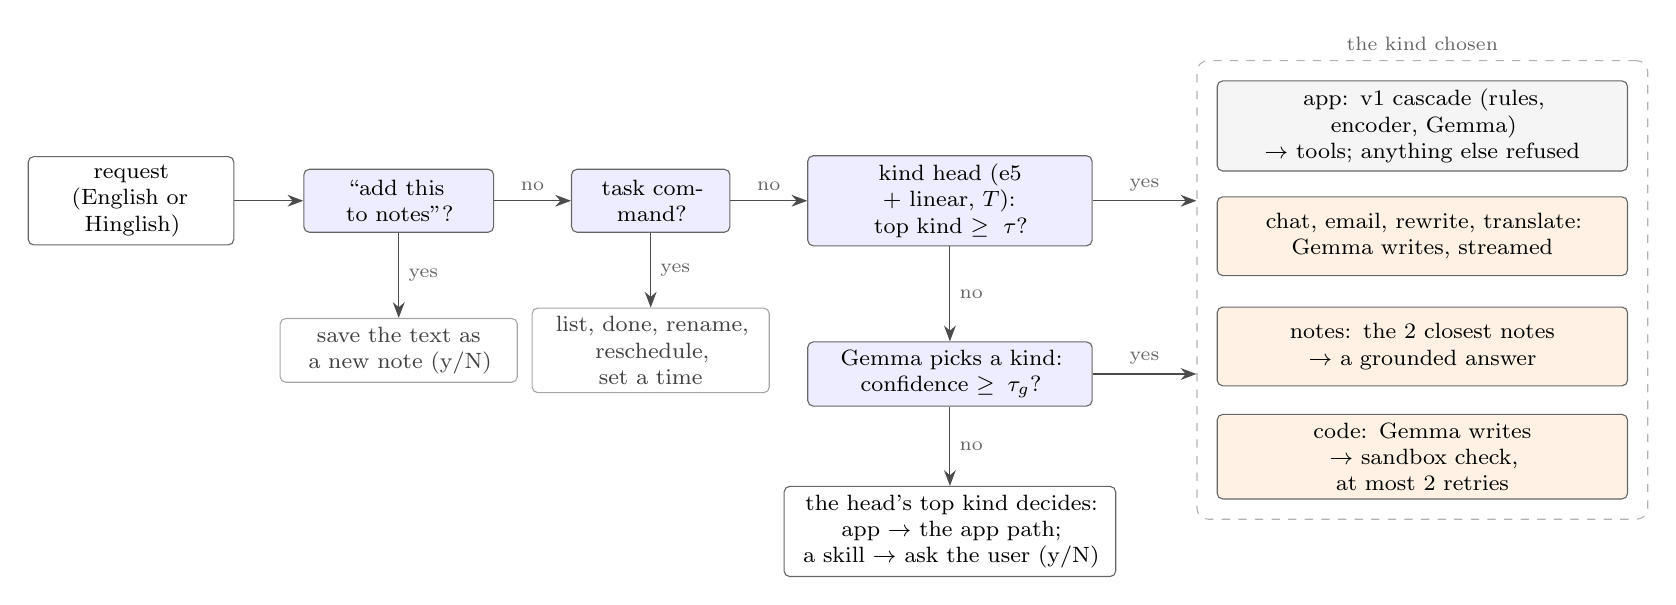
\begin{tikzpicture}[
  font=\footnotesize,
  box/.style={draw=black!60, rounded corners=2pt, align=center, inner sep=3pt, minimum height=8mm},
  act/.style={box, draw=black!35, text=black!75, text width=28mm},
  dec/.style={box, fill=blue!7},
  dest/.style={box, fill=orange!10, text width=50mm, minimum height=10mm},
  arr/.style={-{Stealth[length=2mm]}, black!70},
  lab/.style={font=\scriptsize, text=black!60}]
  \node[box, text width=24mm] (req) at (0,0) {request\\(English or Hinglish)};
  \node[dec, text width=22mm] (save) at (3.4,0) {``add this to notes''?};
  \node[dec, text width=18mm] (cmd) at (6.6,0) {task command?};
  \node[dec, text width=34mm] (head) at (10.4,0) {kind head (e5 + linear, $T$):\\top kind $\ge\tau$?};
  \node[dec, text width=34mm] (gem) at (10.4,-2.2) {Gemma picks a kind:\\confidence $\ge\tau_g$?};
  \node[box, text width=40mm] (last) at (10.4,-4.2) {the head's top kind decides:\\app $\to$ the app path;\\a skill $\to$ ask the user (y/N)};
  \node[act] (saveact) at (3.4,-1.9) {save the text as\\a new note (y/N)};
  \node[act] (cmdact) at (6.6,-1.9) {list, done, rename,\\reschedule, set a time};
  \node[dest, fill=black!4] (app) at (16.4,0.95) {app: v1 cascade (rules, encoder, Gemma)\\$\to$ tools; anything else refused};
  \node[dest] (w) at (16.4,-0.45) {chat, email, rewrite, translate:\\Gemma writes, streamed};
  \node[dest] (qa) at (16.4,-1.85) {notes: the 2 closest notes\\$\to$ a grounded answer};
  \node[dest] (code) at (16.4,-3.25) {code: Gemma writes $\to$ sandbox check,\\at most 2 retries};
  \node[draw=black!30, dashed, rounded corners, fit=(app)(w)(qa)(code), inner sep=2.5mm,
        label={[lab]above:the kind chosen}] (dests) {};
  \draw[arr] (req) -- (save);
  \draw[arr] (save) -- node[lab, above]{no} (cmd);
  \draw[arr] (cmd) -- node[lab, above]{no} (head);
  \draw[arr] (save) -- node[lab, right]{yes} (saveact);
  \draw[arr] (cmd) -- node[lab, right]{yes} (cmdact);
  \draw[arr] (head) -- node[lab, right]{no} (gem);
  \draw[arr] (gem) -- node[lab, right]{no} (last);
  \draw[arr] (head.east) -- node[lab, above]{yes} (head.east -| dests.west);
  \draw[arr] (gem.east) -- node[lab, above]{yes} (gem.east -| dests.west);
\end{tikzpicture}}

\caption{How v3 handles a request. Saving a note (read from the text as typed) and task commands are checked first. If the
kind head's top kind reaches $\tau$, it decides: \emph{app} takes the unchanged app path (v1's cascade and tools), a
skill is written. Below $\tau$, whatever the top kind, Gemma's choice decides if its confidence reaches $\tau_g$;
otherwise the head's top kind decides, except that a skill is proposed to the user as a y/N question.}
\label{fig:arch}
\end{figure}

Figure~\ref{fig:arch} shows the path of a request. Everything runs in one always-on process, \texttt{kestrel serve},
that keeps the rules and the encoder (multilingual-e5-small, 8-bit) loaded and starts the SLM in a worker process on
the first request that needs it, stopping it after ten idle minutes. The terminal client and the browser page talk to
it over a local socket and a localhost HTTP server; answers from the SLM are streamed as they are written, except notes answers and note summaries, which are shown after a
grounding check (Section~\ref{sec:notes}). The research
code paths, the nine-intent ontology, its datasets and its frozen configurations are untouched: v3 adds an application
layer in front of them.

\paragraph{Skills.} \emph{Chat} answers general questions and explanations; every chat answer ends with a visible note
that an offline small model wrote it and may be wrong. Current facts, live data and calculations stay on the app path,
where they are refused. \emph{Email} writes a draft (sending stays an app request). \emph{Rewrite} changes a given text
in its own language, and \emph{translate} puts it into another; a short note after the request names the output
language and script (``hindi'' is written in Devanagari, Hinglish in Latin letters). Answers are capped at 512 tokens
for chat and email and 384 for rewriting and translation, and a capped answer says that it was cut.

\paragraph{The worker's start.} On this laptop Gemma-4-E2B decodes \kv{e0.gemma.tg} tokens per second and reads a
prompt at \kv{e0.gemma.pp} tokens per second (E0, v1's measurement protocol), so long prompts dominate latency. Two
changes make the on-demand worker cheap to start (Section~\ref{sec:res-system}): its weights are memory-mapped instead
of copied, and the key--value state of its \kv{worker.prefix.tokens}-token few-shot prompt prefix is saved to a cache
file after the first start and loaded afterwards, if and only if the saved token list equals the prefix.

\paragraph{Privacy.} No component opens a network connection; the browser page binds to 127.0.0.1 by default and
requires a key for its API. (A wifi-sharing option exists for a trusted local network over plain HTTP and is off.)
Model-written code runs only inside the sandbox of Section~\ref{sec:code}.

% ---------------------------------------------------------------------------------------------------------------
\section{The kind decision}\label{sec:kinds}

\paragraph{Kinds.} A request's kind is \emph{app} (the old path), \emph{chat}, \emph{email}, \emph{rewrite},
\emph{translate}, \emph{notes} (a question that the user's notes answer) or \emph{code} (code to write, fix, shorten or
test; explaining code is chat). The kinds were added in three dataset versions, Kinds-v0 to v2; Table~\ref{tab:datasets} lists the two that were
tested.

\paragraph{Head.} One e5 pass embeds the request (``query:'' prefix), and a multinomial logistic regression head
gives a probability per kind. Its regularization $C$ is chosen on validation macro-F1. Its temperature $T$ is
cross-fitted: train and calibration items are split into \kv{kh2.folds} folds by template family, each fold's logits
come from a head trained on the other folds, and $T$ minimises the negative log-likelihood of all out-of-fold logits; the
final head is then trained on train and calibration together. (On Kinds-v0, a temperature fitted on its
calibration split alone (84 to 103 items) made validation ECE worse in four of five development runs.)

\paragraph{Fallback and asking.} If the head's top kind reaches $\tau$, it decides: \emph{app} goes the old way, a
skill is written. Below $\tau$, Gemma is prompted with the kinds' definitions and two examples per kind and language,
decodes one label under a grammar that allows only the labels, and its confidence (the label's probability,
temperature-scaled on the calibration split by binary cross-entropy, as v1's Tier~4) must reach $\tau_g$ for its kind
to decide. Otherwise the head's top kind decides as before, except that a skill is not written but proposed to the
user as a y/N question. Each decision is therefore one of four outcomes: \emph{right}; \emph{asked}; \emph{sent the old
way} (a skill request taken by the app path, which refuses it or takes it for another action); or \emph{a skill not asked for} (a wrong skill
written).

\paragraph{Choosing $\tau$ and $\tau_g$.} Both were chosen on the validation split, over
$\{0.5,0.6,0.7,0.8,0.9\}^2$, by a rule fixed before the run: fewest wrong decisions (both wrong outcomes), then
fewest questions, then the lower $\tau$ (fewer SLM calls), then the higher $\tau_g$. For Kinds-v1 this gave
$\tau=\kv{fb1.tau}$, $\tau_g=\kv{fb1.taug}$; for Kinds-v2, $\tau=\kv{fb2.tau}$, $\tau_g=\kv{fb2.taug}$
(\kv{fb2.val.right} right on validation). The service uses the Kinds-v2 head and settings.

% ---------------------------------------------------------------------------------------------------------------
\section{Notes by meaning and notes Q\&A}\label{sec:notes}

\paragraph{Retrieval.} Each note is cut into chunks (its title and one paragraph), embedded once with the
``passage:'' prefix and cached by a hash of the note's text. The keyword search of v1 runs first, unchanged; when it
returns fewer than three notes, the single closest note by meaning (a note's score is its best chunk's cosine) is added
if its score reaches $\theta$, labelled ``(by meaning)''. A query that contains a common Hindi word is first put into
English by Gemma. $\theta$ was chosen on development data to maximise the share of queries whose note was found minus
the share of queries without a note that received one.

\paragraph{Q\&A.} A question of kind \emph{notes} retrieves the $N=2$ closest notes, none if even the closest is below
$\theta$. Gemma is told to answer only from them, in the question's language, or to say exactly \texttt{NOT IN NOTES}.
A grounding check then requires every number and name in the answer to occur in the notes. The user sees a grounded
answer with the note it came from, or the reply ``The notes do not say this: so the reply is not available for this
information'' (the author's own wording), or, when the answer could not be checked, the closest note instead.

% ---------------------------------------------------------------------------------------------------------------
\section{The code loop}\label{sec:code}

A request of kind \emph{code} goes to Gemma with a system prompt for short, standard-library Python (at most 640
tokens). The code is then checked in a sandbox: bubblewrap\footnote{\url{https://github.com/containers/bubblewrap}}
with every namespace unshared (so no network), \texttt{/usr} read-only, an empty \texttt{/tmp} and a fresh work folder
as the only writable place, a clean environment and no home directory; inside it, resource limits of 512~MiB of
memory, 10~s of CPU, 10~MiB files and 64 processes, plus a wall-clock timeout, and \texttt{python3 -E -S}. Code is
imported (so it compiles and its top level runs); code that waits for input at its top level is only compiled, since
the sandbox has no input to give it. A syntax error, a crash or a timeout goes back to Gemma with the code, at most two
times. The answer carries one line saying what was checked (``I checked it in a safe sandbox: no errors.'') and a
caveat. The evaluation harness (Section~\ref{sec:res-code}) checks by request type instead: a function or a fix is
imported, a script is only compiled.

The loop deliberately does not run tests written by the model. In the first harness, models were asked to add their
own checks and were retried when those failed; on development data Qwen3-4B's own checks failed on right code (wrong
asserts, or asserts written where a sample input was expected) and caused \kv{code.dev.qbig.retries} retries without
changing a single outcome (Section~\ref{sec:res-code}).

% ---------------------------------------------------------------------------------------------------------------
\section{Data and protocol}\label{sec:setup}

\begin{table}[t]
\centering\small
\caption{The v3 evaluation sets. All are synthetic: drafted with an AI assistant from families of English and
Romanized Hindi (Hinglish) phrasings, and split by family. ``Reviewed'' means reviewed by the author; ``claude
reviewed'' means the author waived the review and the AI assistant reviewed it, with a separate agent judging the files
against written criteria. Kinds-v2's test split contains Kinds-v1's test split plus \kv{kv2.test.fresh} fresh items.}
\label{tab:datasets}
\resizebox{\textwidth}{!}{% Generated by experiments/analysis/paper_assets_v3.py.
\begin{tabular}{llll}
\toprule
Dataset & Labels / content & Items (train / cal / val / test) & Review \\
\midrule
Kestrel-Kinds-v1 & 6 kinds & 920 / 115 / 136 / 256 & reviewed \\
Kestrel-Kinds-v2 & 7 kinds (+ code) & 1000 / 123 / 152 / 280 (24 fresh) & claude reviewed \\
Kestrel-NotesQ-v0 & 18 fixture notes & dev 22 (4 none) / test 20 (2 none) & reviewed \\
Kestrel-NotesQA-v0 & same notes & dev 26 (6 unans.) / test 25 (6 unans.) & reviewed \\
Kestrel-CodeTasks-v0 & 4 types & dev 24 / test 24 (24 families) & claude reviewed \\
\bottomrule
\end{tabular}
}
\end{table}

\paragraph{Datasets.} Table~\ref{tab:datasets} lists the sets. Kestrel-Kinds-v0 to v2 contain \emph{app} items
taken from the train, calibration and validation splits of v1's Kestrel-Intents-v0 (its test split was never read)
plus families on the boundaries (``send an email'' and ``search my notes for the translation'' are app requests), and
families for each skill. Kinds-v0 (\kv{kv0.labels} kinds) was reviewed but never tested: its test was moved to
Kinds-v1, which added \emph{notes}. Kinds-v2 added \kv{kv2.fam.n} families: \kv{kv2.fam.code} code, \kv{kv2.fam.chat} chat (among them
explaining code and poems), \kv{kv2.fam.notes} notes, \kv{kv2.fam.rewrite} rewrite and \kv{kv2.fam.app} app; it keeps
Kinds-v1's rows in their splits and adds \kv{kv2.test.fresh} fresh test items. Kestrel-NotesQ-v0 holds paraphrase
queries that share no keyword with their note, over \kv{notes.fixture} fixture notes (never the user's own), with
queries that no note answers; Kestrel-NotesQA-v0 asks questions about the same notes, answerable ones with their key
facts and unanswerable ones. Kestrel-CodeTasks-v0 has \kv{code.families} families of four types (write a function,
write a script, fix broken code, explain code), each with one English and one Hinglish request and hidden checks:
asserts for functions and fixes, input/output cases for scripts (the last output line must contain the answer as
whole words), and facts that a right explanation contains.

\paragraph{Protocol.} Every choice (head, $C$, $T$, $\tau$, $\tau_g$, $\theta$, prompts, model) was made on development
splits. Each test split was then run once. Unlike v1, this protocol was not
pre-registered as a whole: each step's rule was written down before its own run, sometimes after earlier steps' results
were known (Section~\ref{sec:threats}). Proportions are reported with 95\% Wilson intervals~\citep{wilson1927}, computed
from the logged counts. Timings come from the laptop as found (the memory runs record AC power, CPU boost on and Kestrel's own service idle), not from
v1's controlled protocol, and are comparable only within one log.

% ---------------------------------------------------------------------------------------------------------------
\section{Results}\label{sec:results}

\subsection{The kind decision}\label{sec:res-kinds}

\begin{table}[t]
\centering\small
\caption{Kind decisions on the test splits, each run once. ``Skill req.'' are requests whose gold kind is a skill;
``app req.'' are app requests. A taken decision is right, sent the old way, or a skill not asked for; the rest were
asked.}
\label{tab:kinds}
\resizebox{\textwidth}{!}{% Generated by experiments/analysis/paper_assets_v3.py.
\begin{tabular}{lrrrrrr}
\toprule
 & \multicolumn{3}{c}{right} & & sent the & skill not \\
\cmidrule(lr){2-4}
Policy (test split) & all & skill req. & app req. & asked & old way & asked for \\
\midrule
Kinds-v1, head alone & 206/256 (80.5\%) & 27/76 & 179/180 & 18 & 32 & 0 \\
Kinds-v1, head + Gemma & 220/256 (85.9\%) & 40/76 & 180/180 & 11 & 25 & 0 \\
\midrule
Kinds-v2, head alone & 221/280 (78.9\%) & 40/96 & 181/184 & 37 & 20 & 2 \\
Kinds-v2, head + Gemma & 256/280 (91.4\%) & 78/96 & 178/184 & 13 & 5 & 6 \\
\bottomrule
\end{tabular}
}
\end{table}

\begin{figure}[t]
\centering
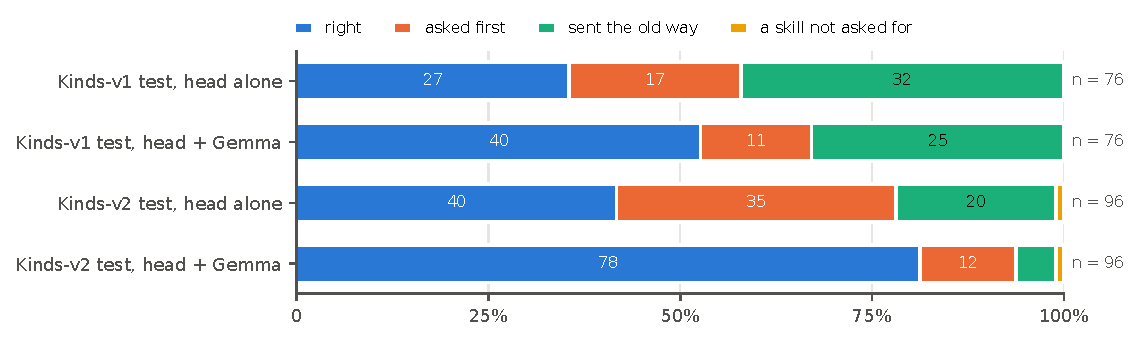
\includegraphics[width=\textwidth]{figures/kinds.pdf}
\caption{Decisions on requests for a skill (test splits). The fallback turns many questions to the user, and some
requests sent the old way, into right answers. On Kinds-v1 a third of skill requests were still sent the old way; on Kinds-v2 most of those are gone, but
\kv{kv1.test} of its \kv{kt2.n} test items had been scored once before (Section~\ref{sec:threats}).}
\label{fig:kinds}
\end{figure}

\begin{table}[t]
\centering\small
\caption{Right decisions per gold kind on the test splits.}
\label{tab:perkind}
% Generated by experiments/analysis/paper_assets_v3.py.
\begin{tabular}{lrrrr}
\toprule
 & \multicolumn{2}{c}{Kinds-v1 test} & \multicolumn{2}{c}{Kinds-v2 test} \\
\cmidrule(lr){2-3}\cmidrule(lr){4-5}
Gold kind & head alone & head + Gemma & head alone & head + Gemma \\
\midrule
app & 179/180 & 180/180 & 181/184 & 178/184 \\
chat & 2/16 & 11/16 & 6/20 & 20/20 \\
code & -- & -- & 1/8 & 7/8 \\
email & 12/16 & 13/16 & 12/16 & 15/16 \\
notes & 1/12 & 1/12 & 7/16 & 12/16 \\
rewrite & 3/16 & 4/16 & 6/20 & 8/20 \\
translate & 9/16 & 11/16 & 8/16 & 16/16 \\
\bottomrule
\end{tabular}

\end{table}

Table~\ref{tab:kinds}, Table~\ref{tab:perkind} and Figure~\ref{fig:kinds} give the test results. On Kinds-v1 the head
alone took \kv{kt1.ha.right} decisions right; with the fallback, \kv{kt1.hg.right} (\kv{kt1.hg.right.pct}, CI
\kv{kt1.hg.right.ci}), with no skill written that was not asked for. Every app request was right (\kv{kt1.hg.app}),
but only \kv{kt1.hg.skill} skill requests were (notes questions \kv{kt1.hg.kind.notes}, rewrite requests
\kv{kt1.hg.kind.rewrite}), and \kv{kt1.hg.sentoldway} skill requests went the old way. Questions about the user's
own people and things (``which floor is the dentist on?'') looked like app requests to both the head and Gemma.

On Kinds-v2, with the fallback, \kv{kt2.hg.right} decisions were right (\kv{kt2.hg.right.pct}, CI
\kv{kt2.hg.right.ci}), \kv{kt2.hg.skill} skill requests among them; \kv{kt2.hg.sentoldway} were sent the old way,
\kv{kt2.hg.notaskedfor} started a skill nobody asked for and \kv{kt2.hg.asked} were asked. The fallback mattered most
for chat and translation: the head alone was right for \kv{kt2.ha.kind.chat} chat and \kv{kt2.ha.kind.translate}
translation requests, the head with Gemma for \kv{kt2.hg.kind.chat} and \kv{kt2.hg.kind.translate}. It cost app
requests a little (\kv{kt2.ha.kind.app} to \kv{kt2.hg.kind.app}): Gemma answered three jokes (``tell me a joke'', ``ek
joke sunao'', ``kuch funny bolo'') and ``google exam preparation'' as chat, which the data label app (small talk and web
searches belong to the app). The head itself, above $\tau$, sent ``london mein abhi kitne baje hain?'' to notes. Rewrite stayed weakest:
\kv{kt2.hg.kind.rewrite} right, most of the others asked first.

The \kv{kv2.test.fresh} fresh items give the cleanest view: \kv{kt2.fresh.hg.right} right with the fallback (CI
\kv{kt2.fresh.hg.right.ci}) against \kv{kt2.fresh.ha.right} for the head alone, which asked
\kv{kt2.fresh.ha.asked} times. English and Hinglish were close (\kv{kt2.hg.en} and \kv{kt2.hg.hi}).

The final heads' validation accuracy was \kv{kh1.val.acc} (Kinds-v1) and \kv{kh2.val.acc} (Kinds-v2), with
macro-F1 \kv{kh1.val.f1} and \kv{kh2.val.f1}; temperature scaling lowered validation ECE from \kv{kh1.val.ece.raw} to
\kv{kh1.val.ece} and from \kv{kh2.val.ece.raw} to \kv{kh2.val.ece}. On test, the Kinds-v2 head reached accuracy
\kv{kt2.head.acc}, macro-F1 \kv{kt2.head.f1} and ECE \kv{kt2.head.ece}; its recall was lowest for chat
(\kv{kt2.head.recall.chat}) and code (\kv{kt2.head.recall.code}). On the validation items where the Kinds-v2 head's top kind
was below $\tau$, Gemma was right \kv{fb2.unsure.gemma} times out of \kv{fb2.unsure.n}, the head \kv{fb2.unsure.head} times.
Gemma's label call took \kv{fb2.ms.p50}\ms\ at the median (p95 \kv{fb2.ms.p95}\ms) on development data, once the
model is loaded; one e5 pass and the head take a few milliseconds (v1 measured the encoder-alone system at a median of
\kv{e1.encoder.median}\ms\ per request).

\subsection{Notes by meaning}\label{sec:res-notes}

\begin{table}[t]
\centering\small
\caption{Retrieval by meaning on Kestrel-NotesQ-v0. Every query's note is missed by the keyword search. ``Right note
added'': the closest note is the query's note and reaches $\theta$. The test split was run once, with $\theta$ from
development.}
\label{tab:notes}
\resizebox{\textwidth}{!}{% Generated by experiments/analysis/paper_assets_v3.py.
\begin{tabular}{lrrrr}
\toprule
Retrieval run & right note added & English & Hinglish & note added to a query with none \\
\midrule
By meaning, no translation (dev, $\theta=0.85$) & 7/18 & 6/9 & 1/9 & 0/4 \\
By meaning, Hinglish via English (dev, $\theta=0.83$) & 18/18 & 9/9 & 9/9 & 0/4 \\
By meaning, Hinglish via English (\textbf{test}, $\theta=0.83$) & 14/18 & 7/9 & 7/9 & 0/2 \\
\bottomrule
\end{tabular}
}
\end{table}

No query's note was found by keywords (by construction), so every success in Table~\ref{tab:notes} is the meaning
search's. Without translation, the right note was the closest one for \kv{md.rank1.en} English but only
\kv{md.rank1.hi} Hinglish development queries, and at the chosen $\theta=\kv{md.theta}$ the search added it for
\kv{md.found.en} and \kv{md.found.hi}. Putting Hinglish queries into English first (``maa ke liye tohfa'' became ``gift
for mother'') made the right note the closest for all \kv{mdt.rank1} development queries, and $\theta=\kv{mdt.theta}$
added it for all of them without adding a note to any of the \kv{notesq.dev.none} queries that have none. On test the
search found \kv{mtt.found} (\kv{mtt.found.pct}, CI \kv{mtt.found.ci}), the same in both languages
(\kv{mtt.found.en} and \kv{mtt.found.hi}), and added no wrong note (\kv{mtt.noise} on queries without a note). The
closest note was right for \kv{mtt.rank1}; for two queries the right note was the closest but just below $\theta$, and ``festival shopping''
ranked the Goa trip above the Diwali shopping note in both languages.

\subsection{Notes Q\&A}

On the test split all \kv{qa.test.all} answers were graded right: \kv{qa.test.ans} answerable questions answered with
their facts and \kv{qa.test.un} unanswerable ones declined (CI \kv{qa.test.all.ci} for the whole split). For every answerable question,
the right note was among the two given. Generating an answer took \kv{qa.test.s.mean}\s\ on average (at most \kv{qa.test.s.max}\s). On development data the same system declined only
\kv{qa.dev.un} unanswerable questions, both before and after the language note described below. Both misses
asked for the price of a cake that the notes mention without a price: Gemma said in its own words that the notes do not
state it, instead of the exact marker, so the app would have shown that sentence as an answer.

The answer's language lagged behind. The test run came before a note that tells Gemma to answer a Hinglish question in
Hinglish; counted afterwards with the same word-list check, \kv{qa.test.hinglish} answered Hinglish test questions got a
Hinglish answer. With the note, \kv{qa.dev.hinglish} did on development data; the test split was not run again.

\subsection{Code}\label{sec:res-code}

\begin{table}[t]
\centering\small
\caption{Kestrel-CodeTasks-v0: requests right after the loop, by type (6 per type), and the mean generation seconds per request (model time; wall time is slightly longer).
The first harness let models add their own tests; the final harness retries only on the sandbox's own errors. In every
run, pass@1 equalled the result after the loop.}
\label{tab:code}
\resizebox{\textwidth}{!}{% Generated by experiments/analysis/paper_assets_v3.py.
\begin{tabular}{lrrrrrr}
\toprule
Model and run & function & script & fix & explain & all & gen.\ s / request \\
\midrule
Gemma-4-E2B, first harness and checks (dev) & 6/6 & 1/6 & 6/6 & 6/6 & 19/24 & 11.1 \\
Qwen3-1.7B, first harness and checks (dev) & 5/6 & 1/6 & 5/6 & 6/6 & 17/24 & 10.4 \\
Qwen3-4B, first harness and checks (dev) & 6/6 & 5/6 & 6/6 & 6/6 & 23/24 & 29.0 \\
\midrule
Gemma-4-E2B, final harness (dev) & 6/6 & 5/6 & 6/6 & 6/6 & 23/24 & 9.1 \\
Gemma-4-E2B, final harness (\textbf{test}, once) & 6/6 & 3/6 & 6/6 & 6/6 & 21/24 & 8.9 \\
\bottomrule
\end{tabular}
}
\end{table}

\begin{figure}[t]
\centering
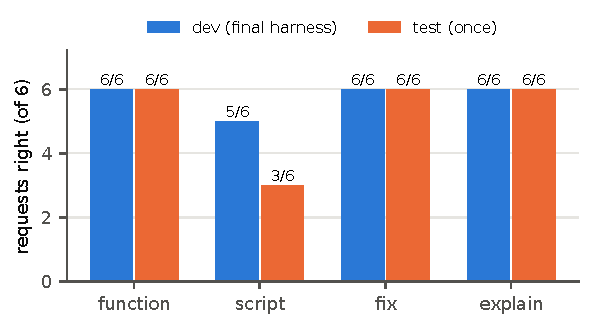
\includegraphics[width=0.62\textwidth]{figures/code.pdf}
\caption{Gemma-4-E2B with the final harness on development data and on the test split (run once).}
\label{fig:code}
\end{figure}

With the first harness (Table~\ref{tab:code}), Qwen3-4B was right \kv{code.dev.qbig.all} times on development data,
Gemma-4-E2B \kv{code.dev.gemma.all} and Qwen3-1.7B \kv{code.dev.qsmall.all}; all of Gemma's misses were scripts
(\kv{code.dev.gemma.script} right). A review of the hidden checks then made script
grading fairer and fix checks stronger, and the same answers rescored to \kv{code.resc.gemma} for Gemma and
\kv{code.resc.qbig} for Qwen3-4B (writing and fixing code: \kv{code.resc.gemma.writefix} vs \kv{code.resc.qbig.writefix}),
at \kv{code.resc.gemma.s} against \kv{code.resc.qbig.s}\s\ of generation per request. Since Qwen3-4B would need a second model in memory
and a second worker, Gemma was kept for code. Its explanations of Hinglish requests were Hinglish
(\kv{code.dev.gemma.explain.hi.hinglish}), against \kv{code.dev.qbig.explain.hi.hinglish} for Qwen3-4B.

With the final harness Gemma was right \kv{code.devfinal.all} times on development data, and on the test split, run
once, \kv{code.test.all} times (\kv{code.test.all.pct}, CI \kv{code.test.all.ci}): all functions
(\kv{code.test.function}), fixes (\kv{code.test.fix}) and explanations (\kv{code.test.explain}), but only
\kv{code.test.script} scripts (Figure~\ref{fig:code}). The failed scripts read input until an uncaught end-of-file
error, stopped at the first blank line, or reversed the line's letters when the Hinglish request (``words ulte order'')
asked for its words in reverse order. Generation took \kv{code.test.s}\s\ per request on average. The sandbox raised no
error in any test answer, so the retry loop never ran (\kv{code.test.retries} retries): its value here is as a check,
not as a repair. Two weaknesses the scores do not show: explanations were asked for in the request's language, but all
three English explanation requests were answered in Hinglish (English: \kv{code.test.explain.en.english}); and the
fact-based grading passed an explanation of a list comprehension that stated a wrong output list.

\subsection{Writing in the right language (development only)}

On \kv{writer.n} development requests for rewriting and translation, a check of the answer's script and
language passed \kv{writer.baseline} with the first prompts and
\kv{writer.final} after the prompts named the output language and a note was added after the request. Translation into
Hindi in Devanagari went from \kv{writer.baseline.translate-hindi} to \kv{writer.final.translate-hindi}; translation
into Hinglish fell from \kv{writer.baseline.translate-hinglish} to \kv{writer.final.translate-hinglish} (the English
text came back unchanged). The prompts were changed while looking at these items, so these scores are optimistic.

\subsection{System costs}\label{sec:res-system}

\begin{table}[t]
\centering\small
\caption{Gemma-4-E2B (Q4\_0) loaded with its weights copied or memory-mapped, page cache cold or warm (median of 3
runs each; one session). Output text was byte-identical in all runs.}
\label{tab:systems}
% Generated by experiments/analysis/paper_assets_v3.py.
\begin{tabular}{llrrrr}
\toprule
Weights & page cache & load (ms) & first token (ms) & anonymous (MiB) & file-backed (MiB) \\
\midrule
copied & cold & 3656 & 111 & 3247 & 8 \\
copied & warm & 2596 & 103 & 3247 & 8 \\
mapped & cold & 2477 & 111 & 1144 & 2702 \\
mapped & warm & 1383 & 117 & 1144 & 2702 \\
\bottomrule
\end{tabular}

\end{table}

\begin{figure}[t]
\centering
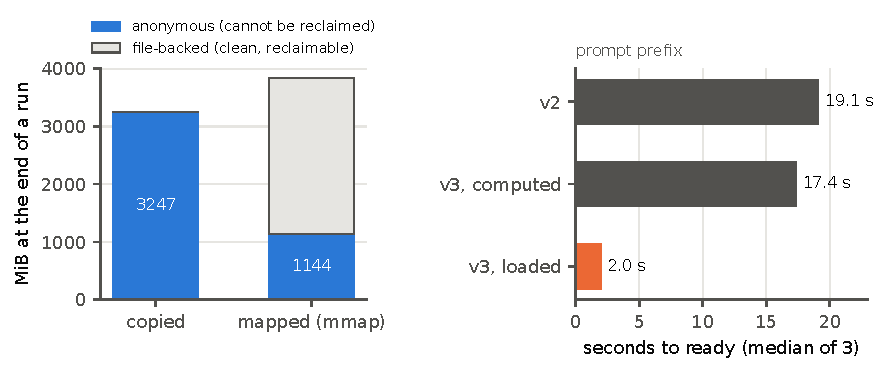
\includegraphics[width=\textwidth]{figures/memory.pdf}
\caption{Left: memory at the end of a run, copied vs mapped weights. Right: time until the service's Gemma worker is
ready, for the v2 worker and the v3 worker with its prompt prefix computed or loaded from the cache.}
\label{fig:memory}
\end{figure}

Mapping the weights cut anonymous memory, which the kernel cannot reclaim, from \kv{mmap.copy.cold.anon} to
\kv{mmap.map.cold.anon}\MiB\ (\kv{mmap.anon.saved}\MiB, \kv{mmap.anon.cut}); the rest of the file,
\kv{mmap.map.cold.file}\MiB, is file-backed and clean (Table~\ref{tab:systems}, Figure~\ref{fig:memory}). Peak-RSS
counters still count those pages, so measured that way the mapped process looks larger. Loading became faster (cold
\kv{mmap.copy.cold.load} to \kv{mmap.map.cold.load}\ms; warm \kv{mmap.copy.warm.load} to \kv{mmap.map.warm.load}\ms),
and the first token came after \kv{mmap.first.min}--\kv{mmap.first.max}\ms\ in every condition. The model's per-layer
embeddings, almost half of the file, are still read at load: the installed llama.cpp binding has no setter for the lazy
mode.

Loading is only part of a cold start. The service's worker primes a \kv{worker.prefix.tokens}-token few-shot prefix
before it can answer. The v2 worker was ready after \kv{worker.v2.s}\s\ (median of \kv{worker.v2.n}); the v3 worker,
computing and saving the prefix, after \kv{worker.miss.s}\s; and loading the saved prefix, after \kv{worker.hit.s}\s,
\kv{worker.speedup} times faster than v2, with \kv{worker.hit.anon}\MiB\ of anonymous memory at ready against
\kv{worker.v2.anon}\MiB.

\subsection{Acceptance run}

Before the version was frozen, every goal feature was driven end to end on a scratch service with the fixture notes.
Over the socket, \kv{acc.socket} requests passed (tasks with times in English and Hinglish, task commands, keyword and
meaning search, summaries, memory, chat, email, rewrite, translation, notes Q\&A, code, saving a note, refusals and the
cut-off note); a first run had passed \kv{acc.run1}, with two failures caused by wrong checks in the script, which were
corrected before a fresh rerun. The browser page passed \kv{acc.page.headless} steps in headless Chrome and
\kv{acc.page.headed} in a visible window, including the Copy button read back from the clipboard. A reminder due at
\kv{acc.reminder.due} was shown \kv{acc.reminder.late}\s\ after its minute began. The automated suites passed
(\kv{acc.cargo} Rust tests, \kv{acc.pytest} Python tests, \kv{acc.bwrap} sandbox tests and \kv{acc.worker} model-worker
tests).

The two failures are the limitations that matter most. ``How much is my rent?'' was refused: the head gave app
0.62, below $\tau$, Gemma also chose app, and the question never reached notes Q\&A, which answers it correctly when it
does. ``Which preferences have I set?'' found nothing, because the memory search of v2 matches stored words. In this run
\kv{acc.fast} requests (\kv{acc.fast.pct}) were answered in under a second: the greeting, creating and deleting a task, task
commands, keyword and English meaning search, opening a document, memory, saving a note and a refusal (median
\kv{acc.fast.median}\s); a translation took \kv{acc.s.tohindi}--\kv{acc.s.toenglish}\s, an email
\kv{acc.s.emailhi}--\kv{acc.s.email}\s, a notes answer \kv{acc.s.qa}\s\ and a written function \kv{acc.s.codefn}\s\ (one run, not a
benchmark: these times include whatever the worker was doing, such as starting).

% ---------------------------------------------------------------------------------------------------------------
\section{Discussion}\label{sec:discussion}

\paragraph{Ask, fall back, or refuse.} The four-outcome view made the trade-offs visible. A higher $\tau$ turns wrong
decisions into questions; the SLM fallback answers many of those questions itself (questions to the user fell from
\kv{kt2.ha.asked} to \kv{kt2.hg.asked} on Kinds-v2, from \kv{kt1.ha.asked} to \kv{kt1.hg.asked} on Kinds-v1), at the
cost of about half a second (Section~\ref{sec:res-kinds}) and occasional confident mistakes on the app's boundary
(jokes, web searches). On Kinds-v1, sending a skill request the old way was by far the most common failure
(\kv{kt1.hg.sentoldway}, against \kv{kt1.hg.notaskedfor} skills not asked for); with Kinds-v2 the two were close
(\kv{kt2.hg.sentoldway} and \kv{kt2.hg.notaskedfor}). The old way is the costlier failure for the user, since the
app path refuses the request or takes it for another action, and nothing tells them that a skill exists.

\paragraph{Data and settings changed together.} Right decisions on skill requests rose from \kv{kt1.hg.skill} on
Kinds-v1 to \kv{kt2.hg.skill} on Kinds-v2, but new families, a new Gemma prompt and new thresholds came together, and no
run separates their effects. The rent question shows the limit of what synthetic families
cover: the Q\&A component answers it, but the decision never sends it there.

\paragraph{A 2B-class model is enough for small, well-specified code, not for I/O.} Gemma matched the larger Qwen3-4B
on our rescored development data in well under half of its time, and on test wrote every function and fix right. Scripts that
read input are its weak spot, and the sandbox cannot catch them, because it has no input to give: it only proves that
code compiles or imports.

\paragraph{Calibration still pays, unevenly.} Cross-fitted temperatures lowered validation ECE for both heads, and the
Kinds-v2 head's test ECE was \kv{kt2.head.ece} (validation: \kv{kh2.val.ece}). But calibration cannot help where the data has no
family: for the rent question both the head (below $\tau$) and Gemma's fallback chose app.

% ---------------------------------------------------------------------------------------------------------------
\section{Threats to Validity}\label{sec:threats}

\paragraph{Internal.} Thresholds, prompts and the code model were chosen on development data, and each test split was
run once. But the protocol grew step by step: Kinds-v2's new families were written after Kinds-v1's test errors were
known, and \kv{kv1.test} of Kinds-v2's \kv{kt2.n} test items are Kinds-v1's test items, so the Kinds-v2 result on those
items is optimistic; the \kv{kv2.test.fresh} fresh items are the clean measure. The prompt changes for answer language
were made while looking at development items. The code model was chosen after the checks were revised on the same
development answers.

\paragraph{Construct.} Explanations are judged by required facts, which a wrong statement can pass. Script grading
reads the last output line. Notes Q\&A grades were assigned by the evaluation script's rules and the author's review
of the sets, not by a second annotator. Language is judged by a word list.

\paragraph{External.} Every set is small (\kv{notesq.test.q} to \kv{kt2.n} test items), synthetic, drafted with an AI
assistant, and about one imagined user's life; two sets were reviewed by the assistant and an independent agent, not
by the author. The notes are \kv{notes.fixture} fixture files. One laptop, one SLM, one encoder; timings were taken on
the laptop as found.

\paragraph{Statistical.} Intervals are wide: \kv{code.test.all} has a 95\% interval of \kv{code.test.all.ci}, and
\kv{qa.test.all} of \kv{qa.test.all.ci}. No hypothesis test was planned, and none is reported.

% ---------------------------------------------------------------------------------------------------------------
\section{Limitations and Future Work}\label{sec:limits}

The acceptance run's README lists \kv{acc.limits} known limitations, frozen with the version. Beyond the two failures
above: requests to write a program ``to solve X'' go to chat (the program comes, unchecked); rewrite requests are often
asked first; jokes go to chat and a time question to notes; Markdown is shown as typed; some notes answers to Hinglish
questions are English; code uses the standard library only and is never run with input; the page can be shared on a
wifi over plain HTTP when the user turns that on; and there is no memory of the conversation, so ``continue'' does not
see the last answer. Energy was not measured.

The next round should start from the user's own misrouted requests: a Kinds-v3 and a CodeTasks-v1 built from them,
reviewed by the author, with a fresh test split. A larger machine (v4) would allow larger models; on this laptop Qwen3-4B
already decodes only \kv{e0.qbig.tg} tokens per second.

% ---------------------------------------------------------------------------------------------------------------
\section{Ethical Considerations}\label{sec:ethics}

All inference runs on the user's machine, and the evaluation used fixture notes, never the user's own. Model-written
code runs only in the sandbox, which has no network and no access to the user's files. Chat answers carry a note that
an offline small model may be wrong, and notes answers name the note they came from. The page's wifi option exposes the
notes to anyone on that network who has the link or can read its traffic; it is off by default and was off when this
paper was written. The data sets and much of the code were drafted with an AI coding assistant and describe no real
person.

% ---------------------------------------------------------------------------------------------------------------
\section{Conclusion}\label{sec:conclusion}

A single 4-bit 2B-class model and a frozen encoder were enough to turn an intent classifier into an offline assistant
that writes, translates, answers from the user's notes and writes small checked programs on an ordinary laptop. The
decisive pieces were cheap: a calibrated head with a model fallback and a question to the user, translation before
retrieval, an explicit ``not in your notes'', a sandbox that checks what it can, and two systems changes that make an
always-on service start in about \kv{worker.hit.s}\s. The weak pieces are recognition of personal questions and rewrite
requests, scripts that read input, and the language of some answers; they need real users' requests rather than more
synthetic families.

\paragraph{Reproducibility.} The system, its data sets, configurations and logs are in the repository at tag
\texttt{v3-frozen}; this paper and its generator were added in a later commit on the same branch. Every measured value,
share, interval and table entry in this paper is generated from the committed logs by
\path{experiments/analysis/paper_assets_v3.py}; configuration constants (token caps, sandbox limits, $N$) and a few
small counts in the prose (such as the number of development runs or of misrouted requests named) are typed and were
checked by hand. \path{paper/v3/number_check.md}
records independent re-derivations of the numbers and claims, with the corrections they led to.

\bibliographystyle{plainnat}
\bibliography{../references,references_v3}

\end{document}
